

\section{Anhang Software}
Im folgenden Kapitel ist die von uns geschriebene Software dokumentiert.




\subsection{main.c}
\lstinputlisting{ProjArbBautAutomat-master/src/main.c}

\begin{figure}[h]
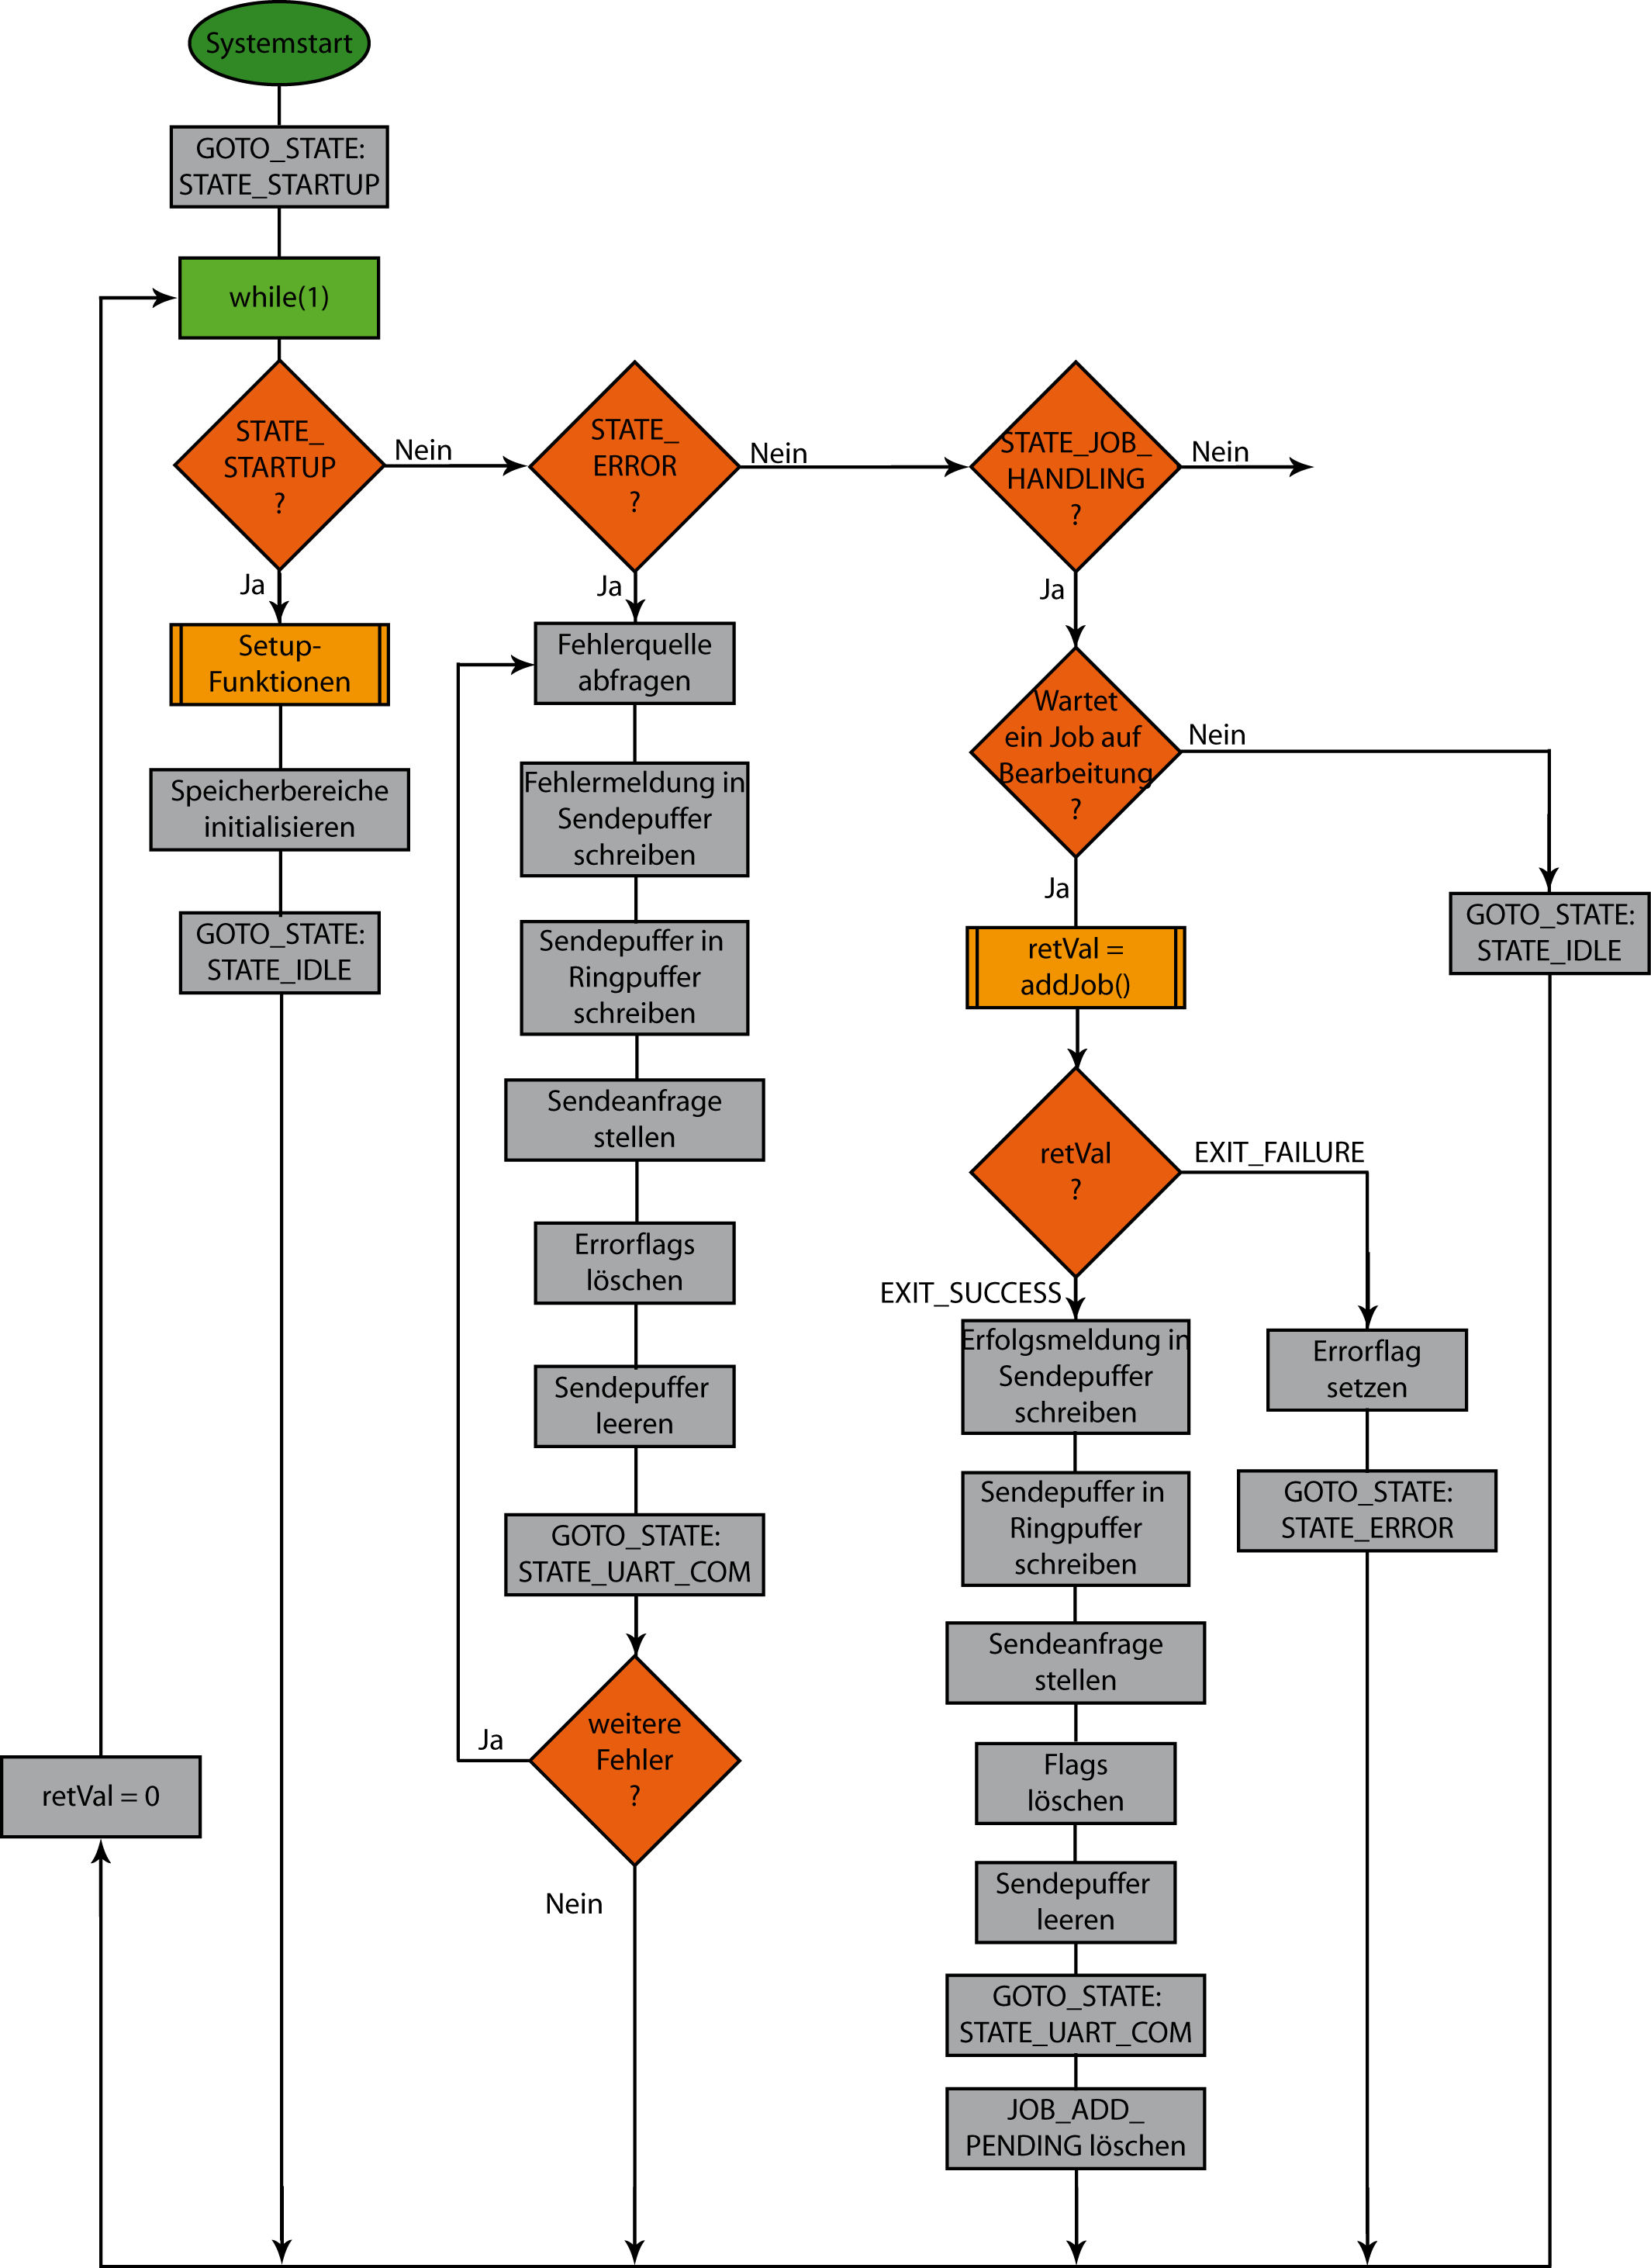
\includegraphics[scale = 0.8]{./main1.png}
\hspace{-14pt}
\caption{Ablaufdiagramm der main, teil 1}
\end{figure} 

\begin{figure}[h]
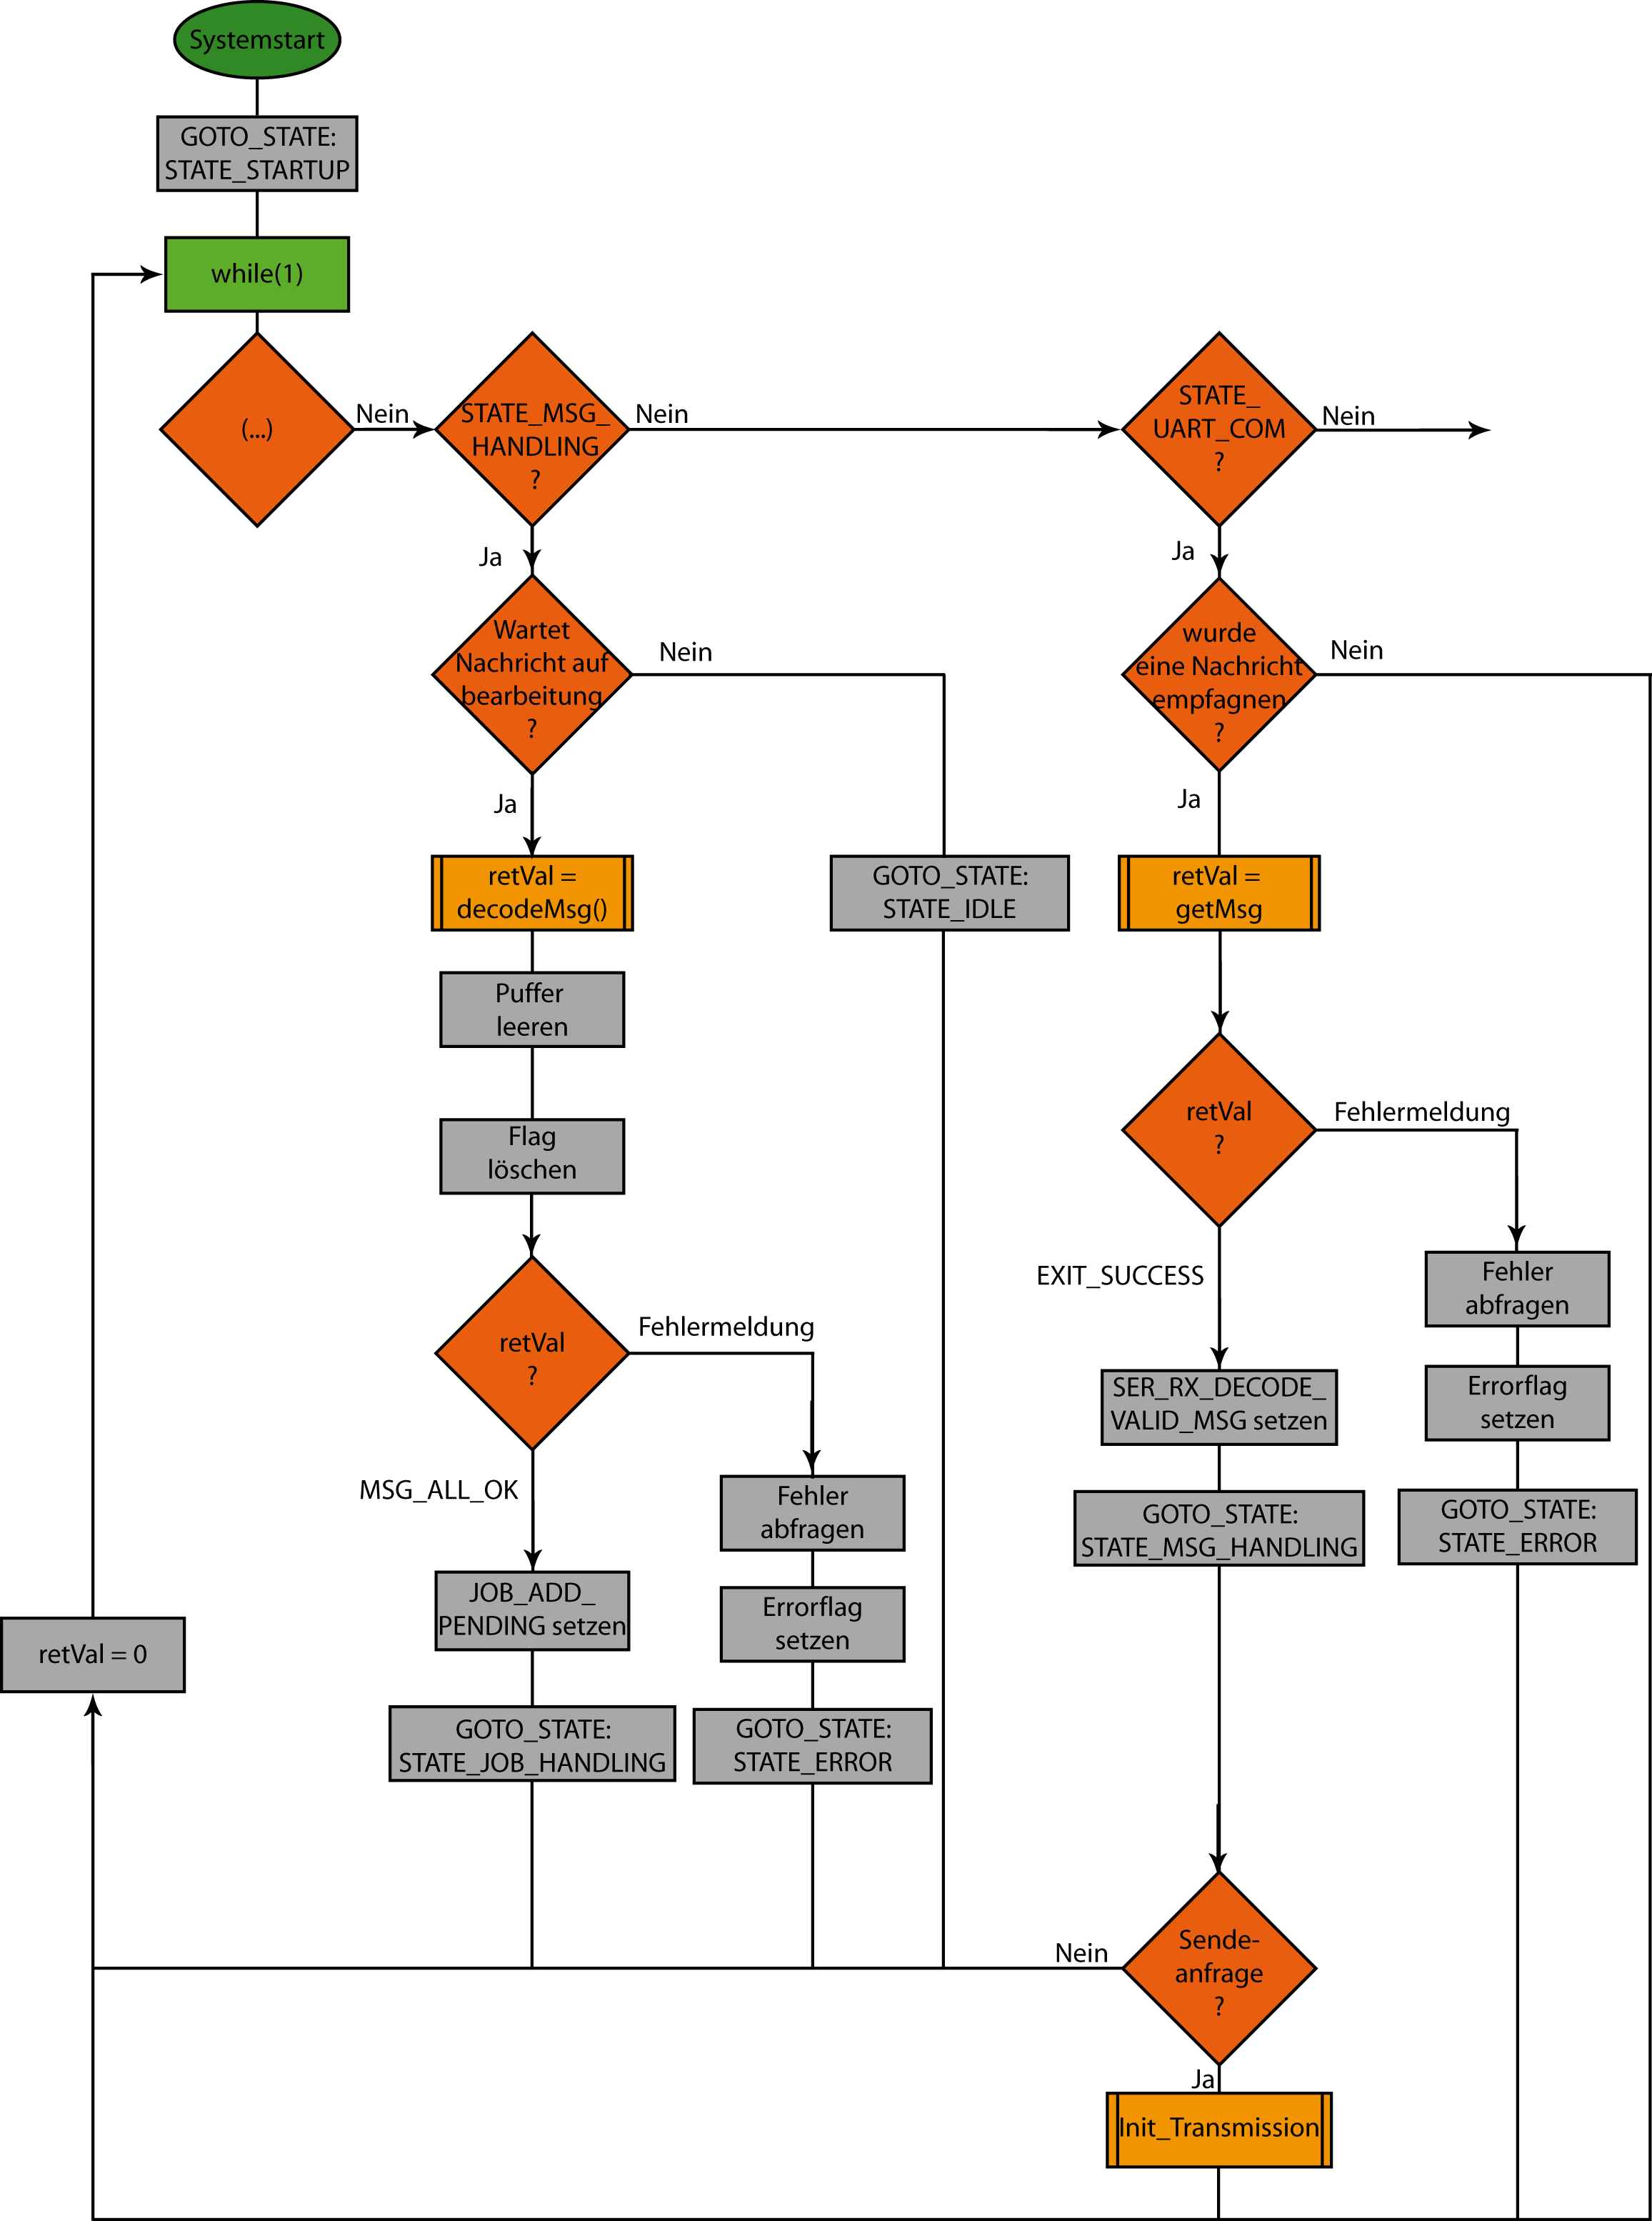
\includegraphics[scale = 0.8]{./main2.png}
\hspace{-14pt}
\caption{Ablaufdiagramm der main, teil 2}
\end{figure} 

\begin{figure}[h]
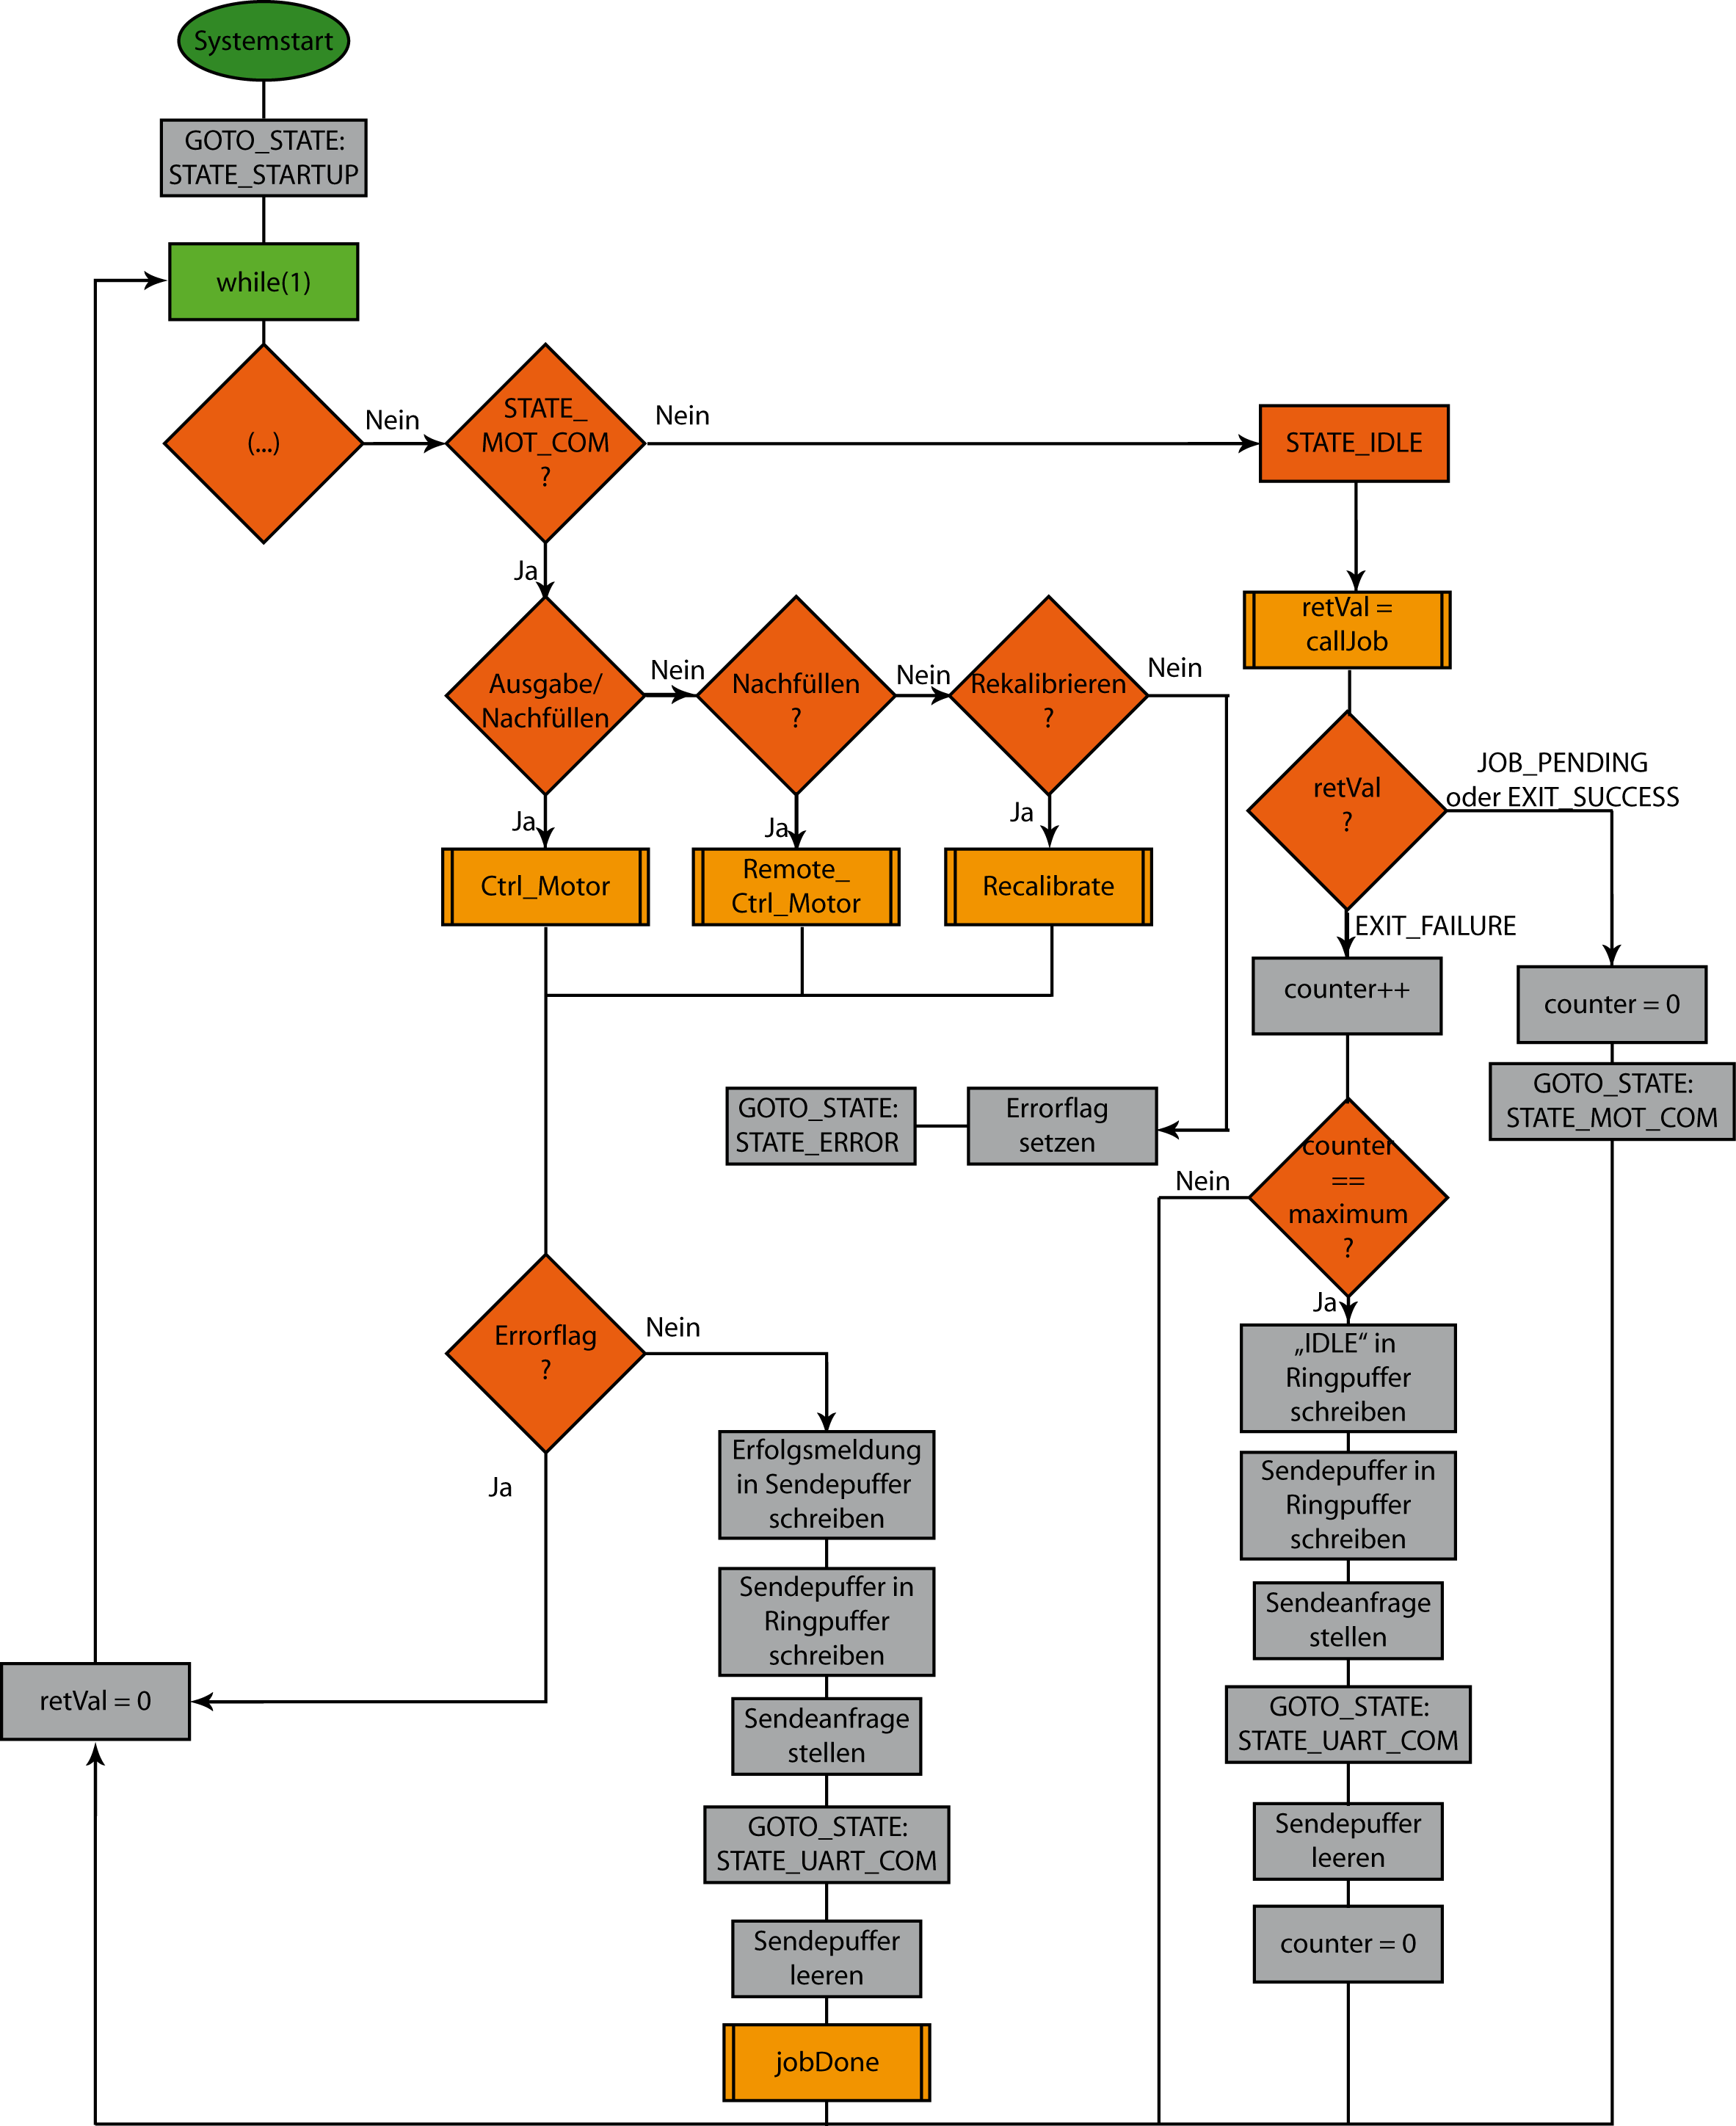
\includegraphics[scale = 0.8]{./main3.png}
\hspace{-14pt}
\caption{Ablaufdiagramm der main, teil 3}
\end{figure} 

\begin{figure}[h]
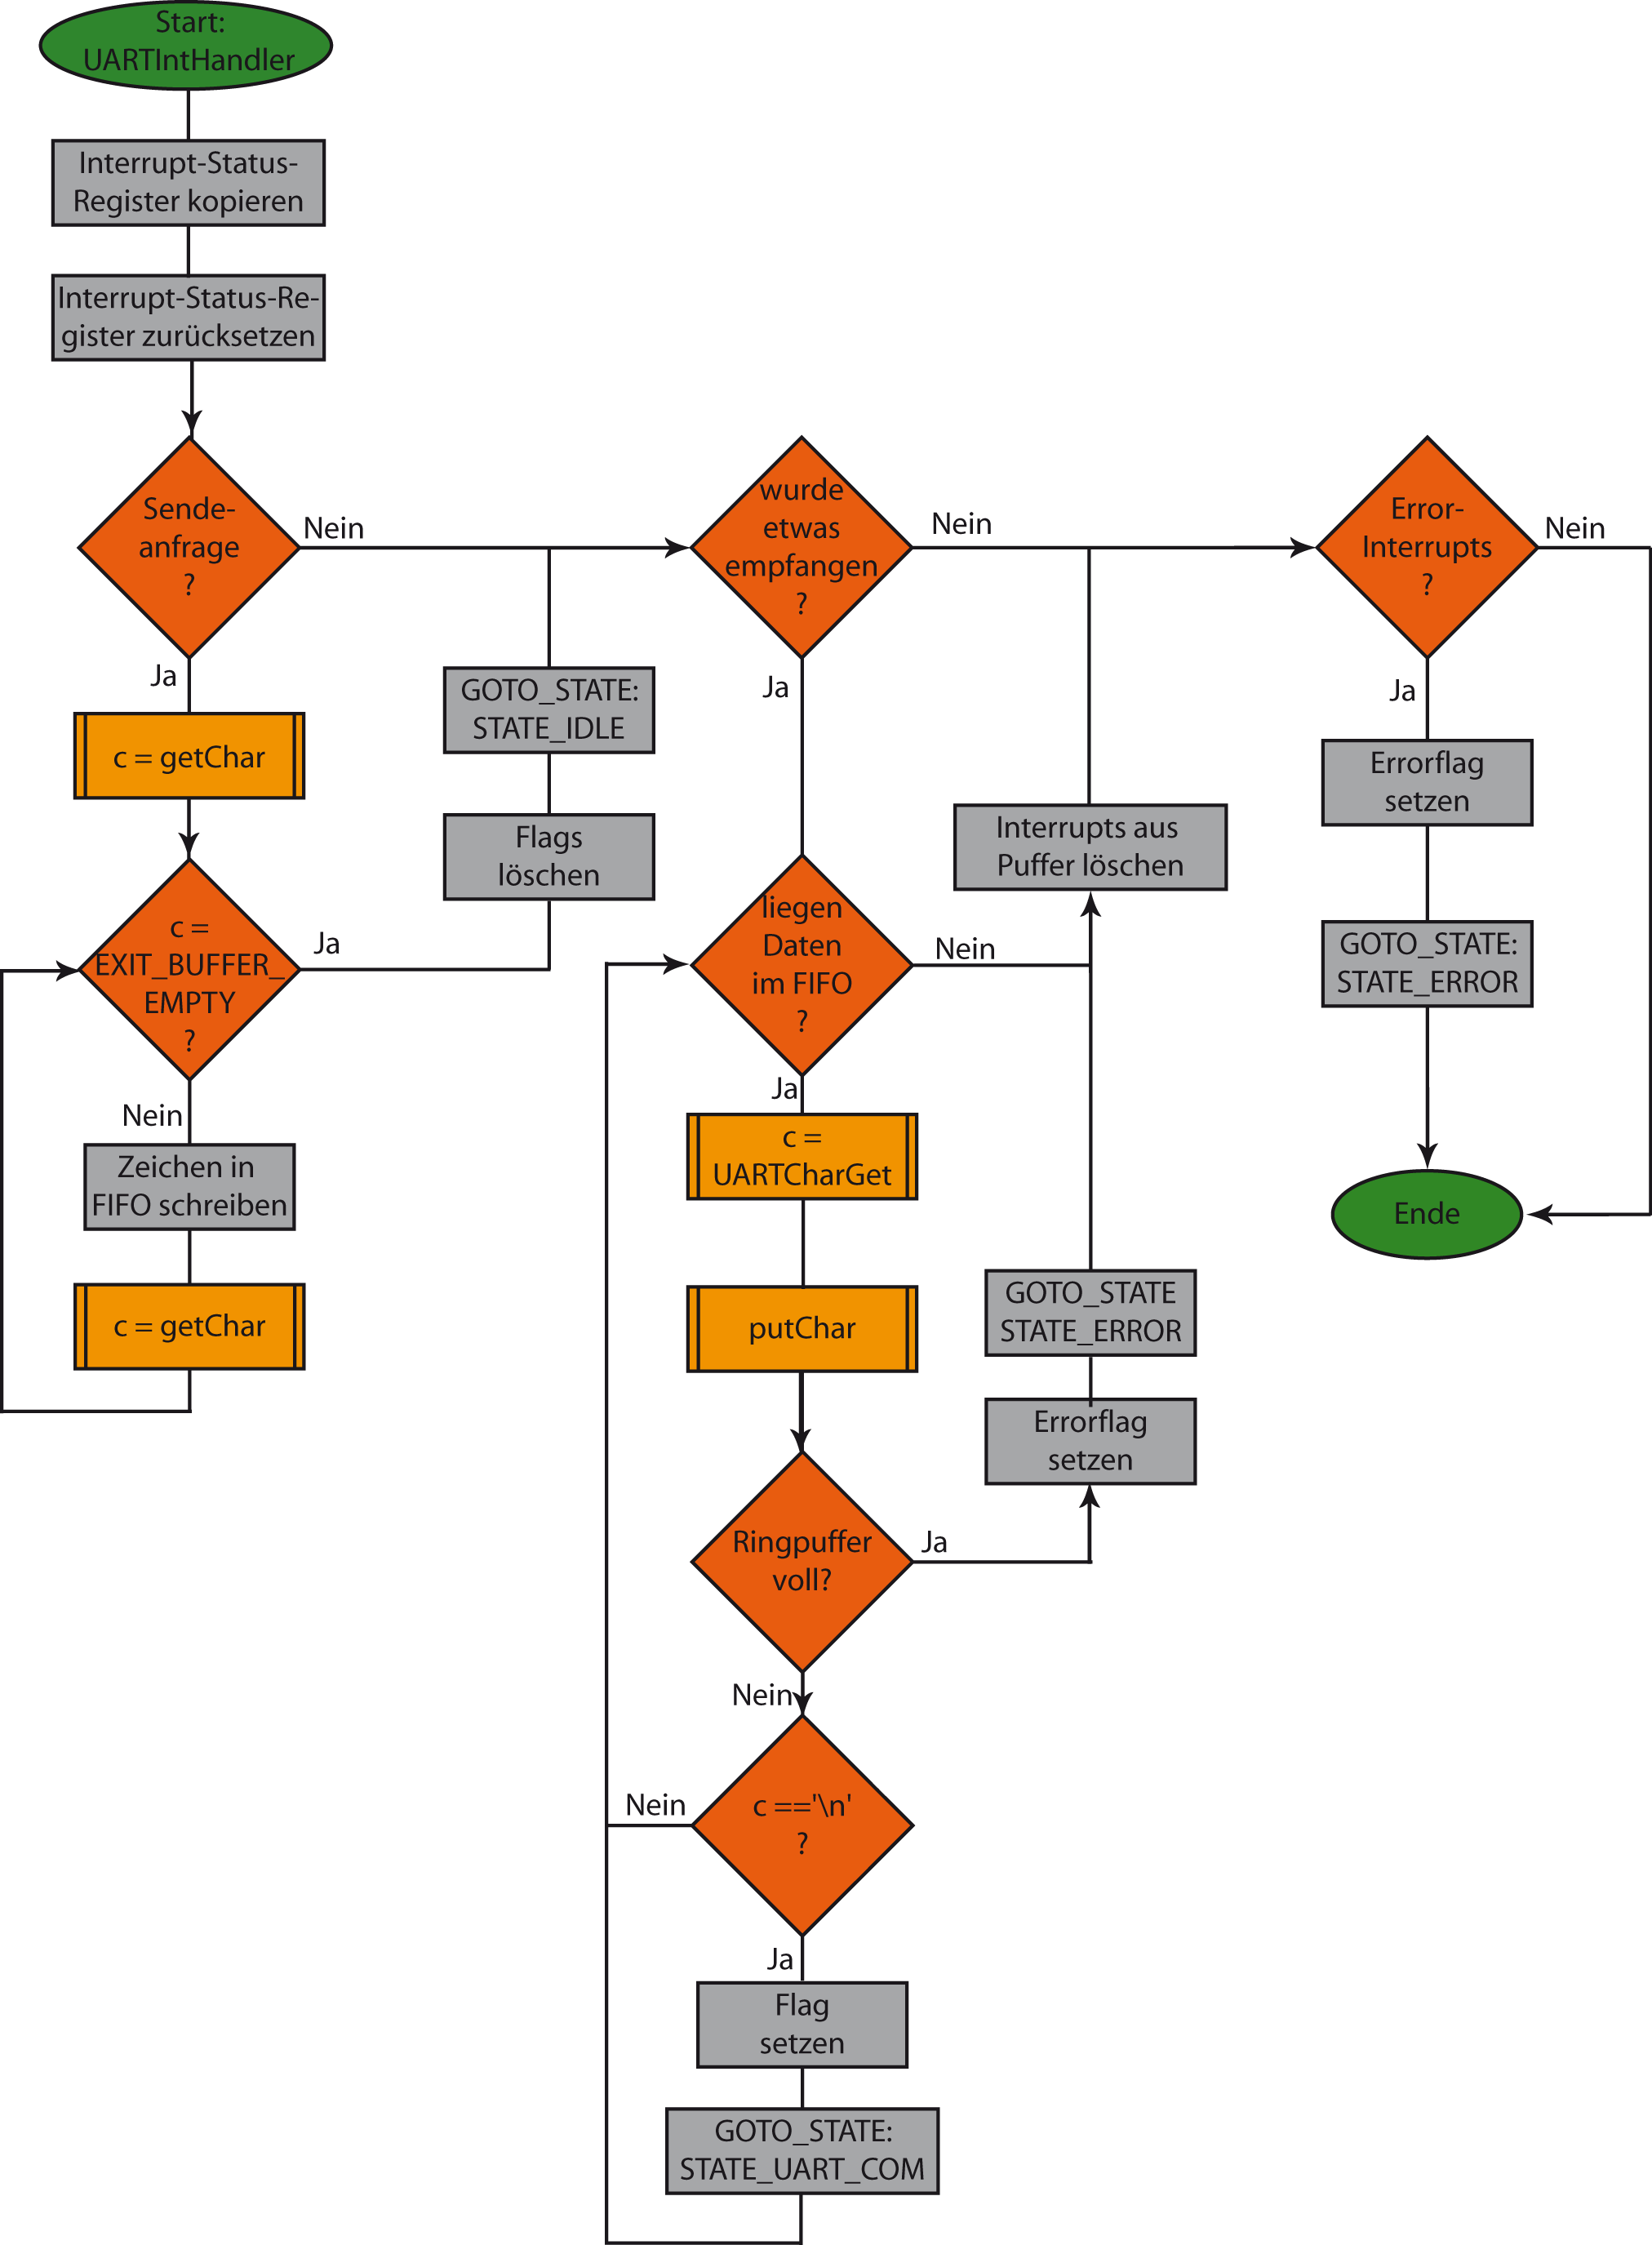
\includegraphics[scale = 0.8]{./ISR.png}
\hspace{-14pt}
\caption{Ablaufdiagramm der Interrupt Service Routine für die UART-Schnittstelle}
\end{figure} 

\begin{figure}[h]
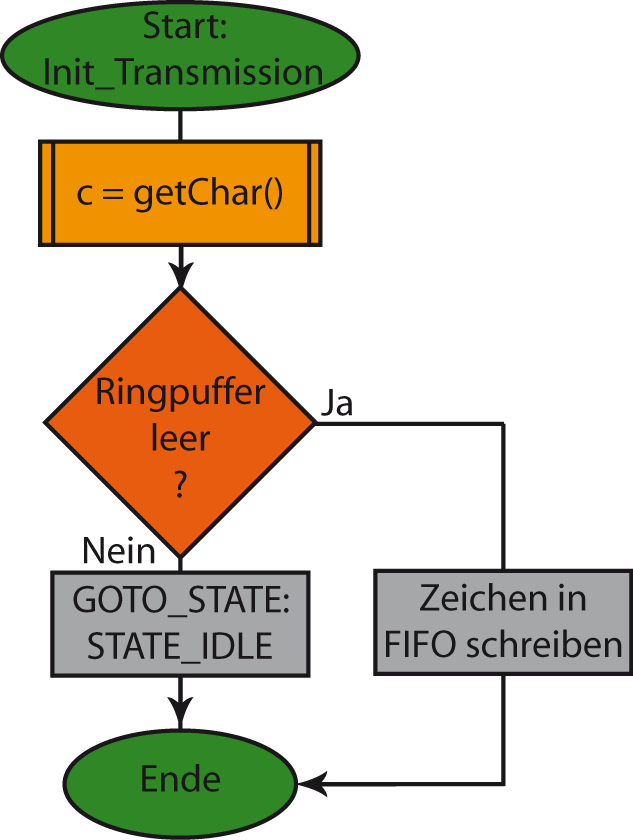
\includegraphics[scale = 0.8]{./Init_Transmission.png}
\hspace{-14pt}
\caption{Ablaufdiagramm der Funktion Init\_Transmission}
\end{figure} 


\begin{figure}[h]
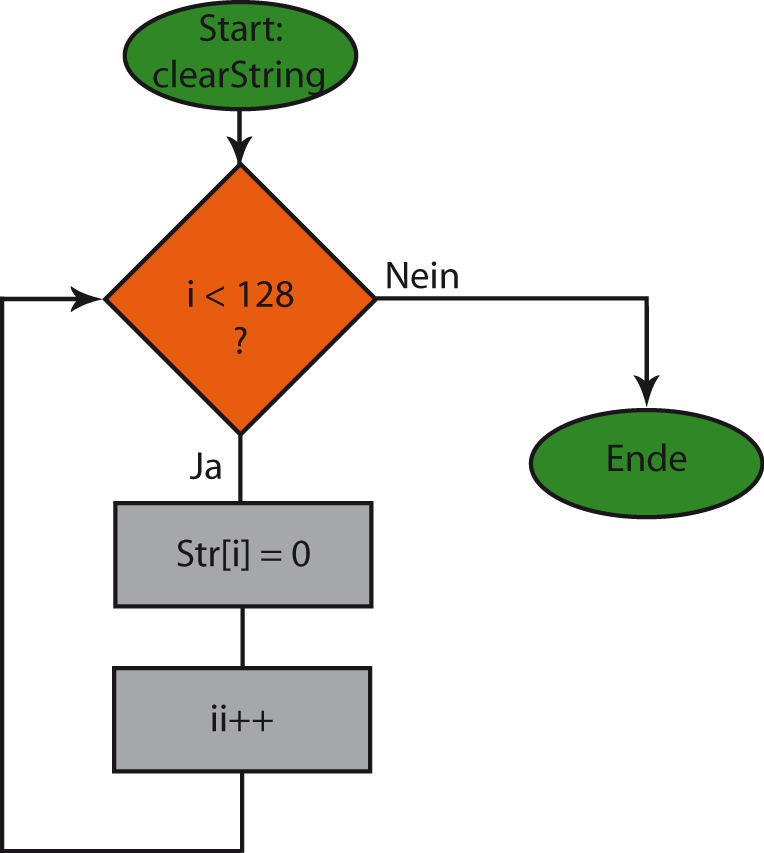
\includegraphics[scale = 0.8]{./Clear_String.png}
\hspace{-14pt}
\caption{Ablaufdiagramm der Funktion clearString}
\end{figure} 

\begin{figure}[h]
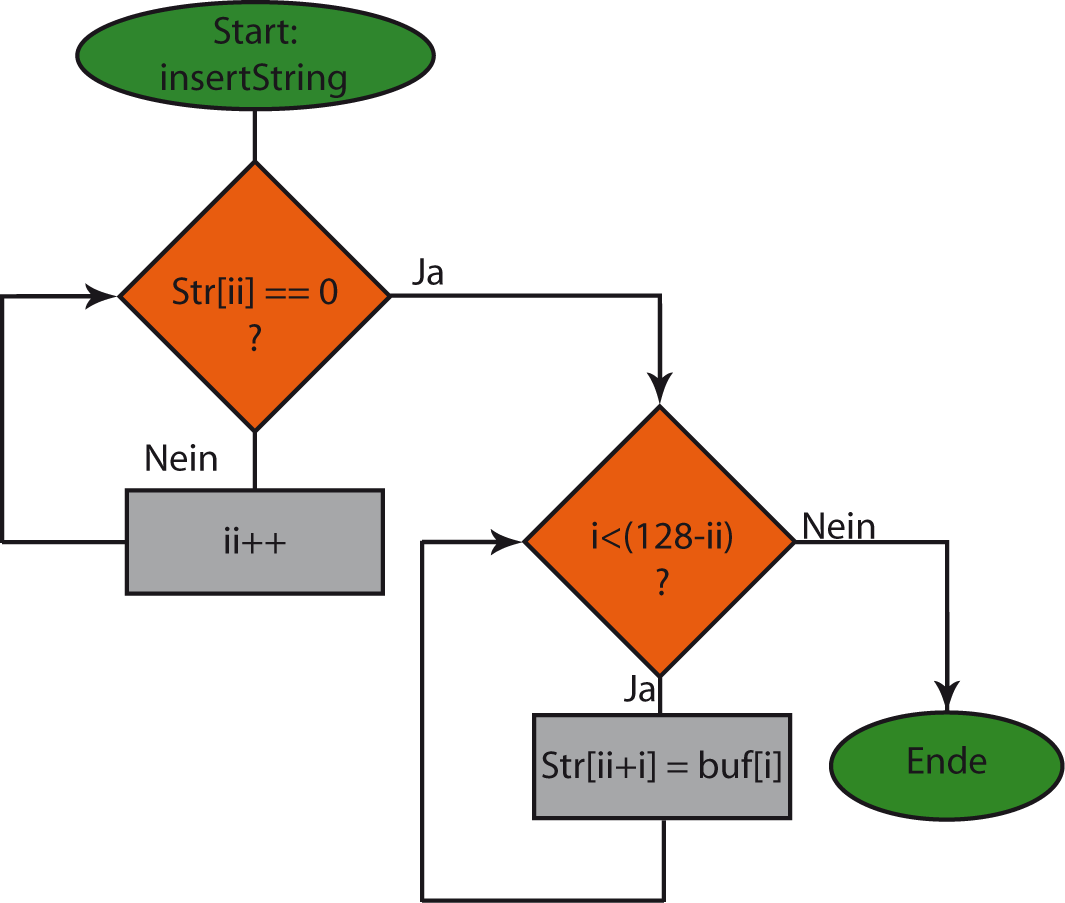
\includegraphics[scale = 0.8]{./Insert_String.png}
\hspace{-14pt}
\caption{Ablaufdiagramm der Funktion insertString}
\end{figure} 







\subsection{main.h}
\lstinputlisting{ProjArbBautAutomat-master/inc/main.h}








\subsection{circular.c}
\lstinputlisting{ProjArbBautAutomat-master/src/circular.c}
\begin{figure}[h]
\includegraphics[scale = 0.8]{./getchar.png}
\hspace{-14pt}
\caption{Ablaufdiagramm der Funktion getChar}
\end{figure} 

\begin{figure}[h]
\includegraphics[scale = 0.8]{./putchar.png}
\hspace{-14pt}
\caption{Ablaufdiagramm der Funktion putChar}
\end{figure} 

\begin{figure}[h]
\includegraphics[scale = 0.8]{./getrembufspace.png}
\hspace{-14pt}
\caption{Ablaufdiagramm der Funktion getRemBufSpace}
\end{figure} 

\begin{figure}[h]
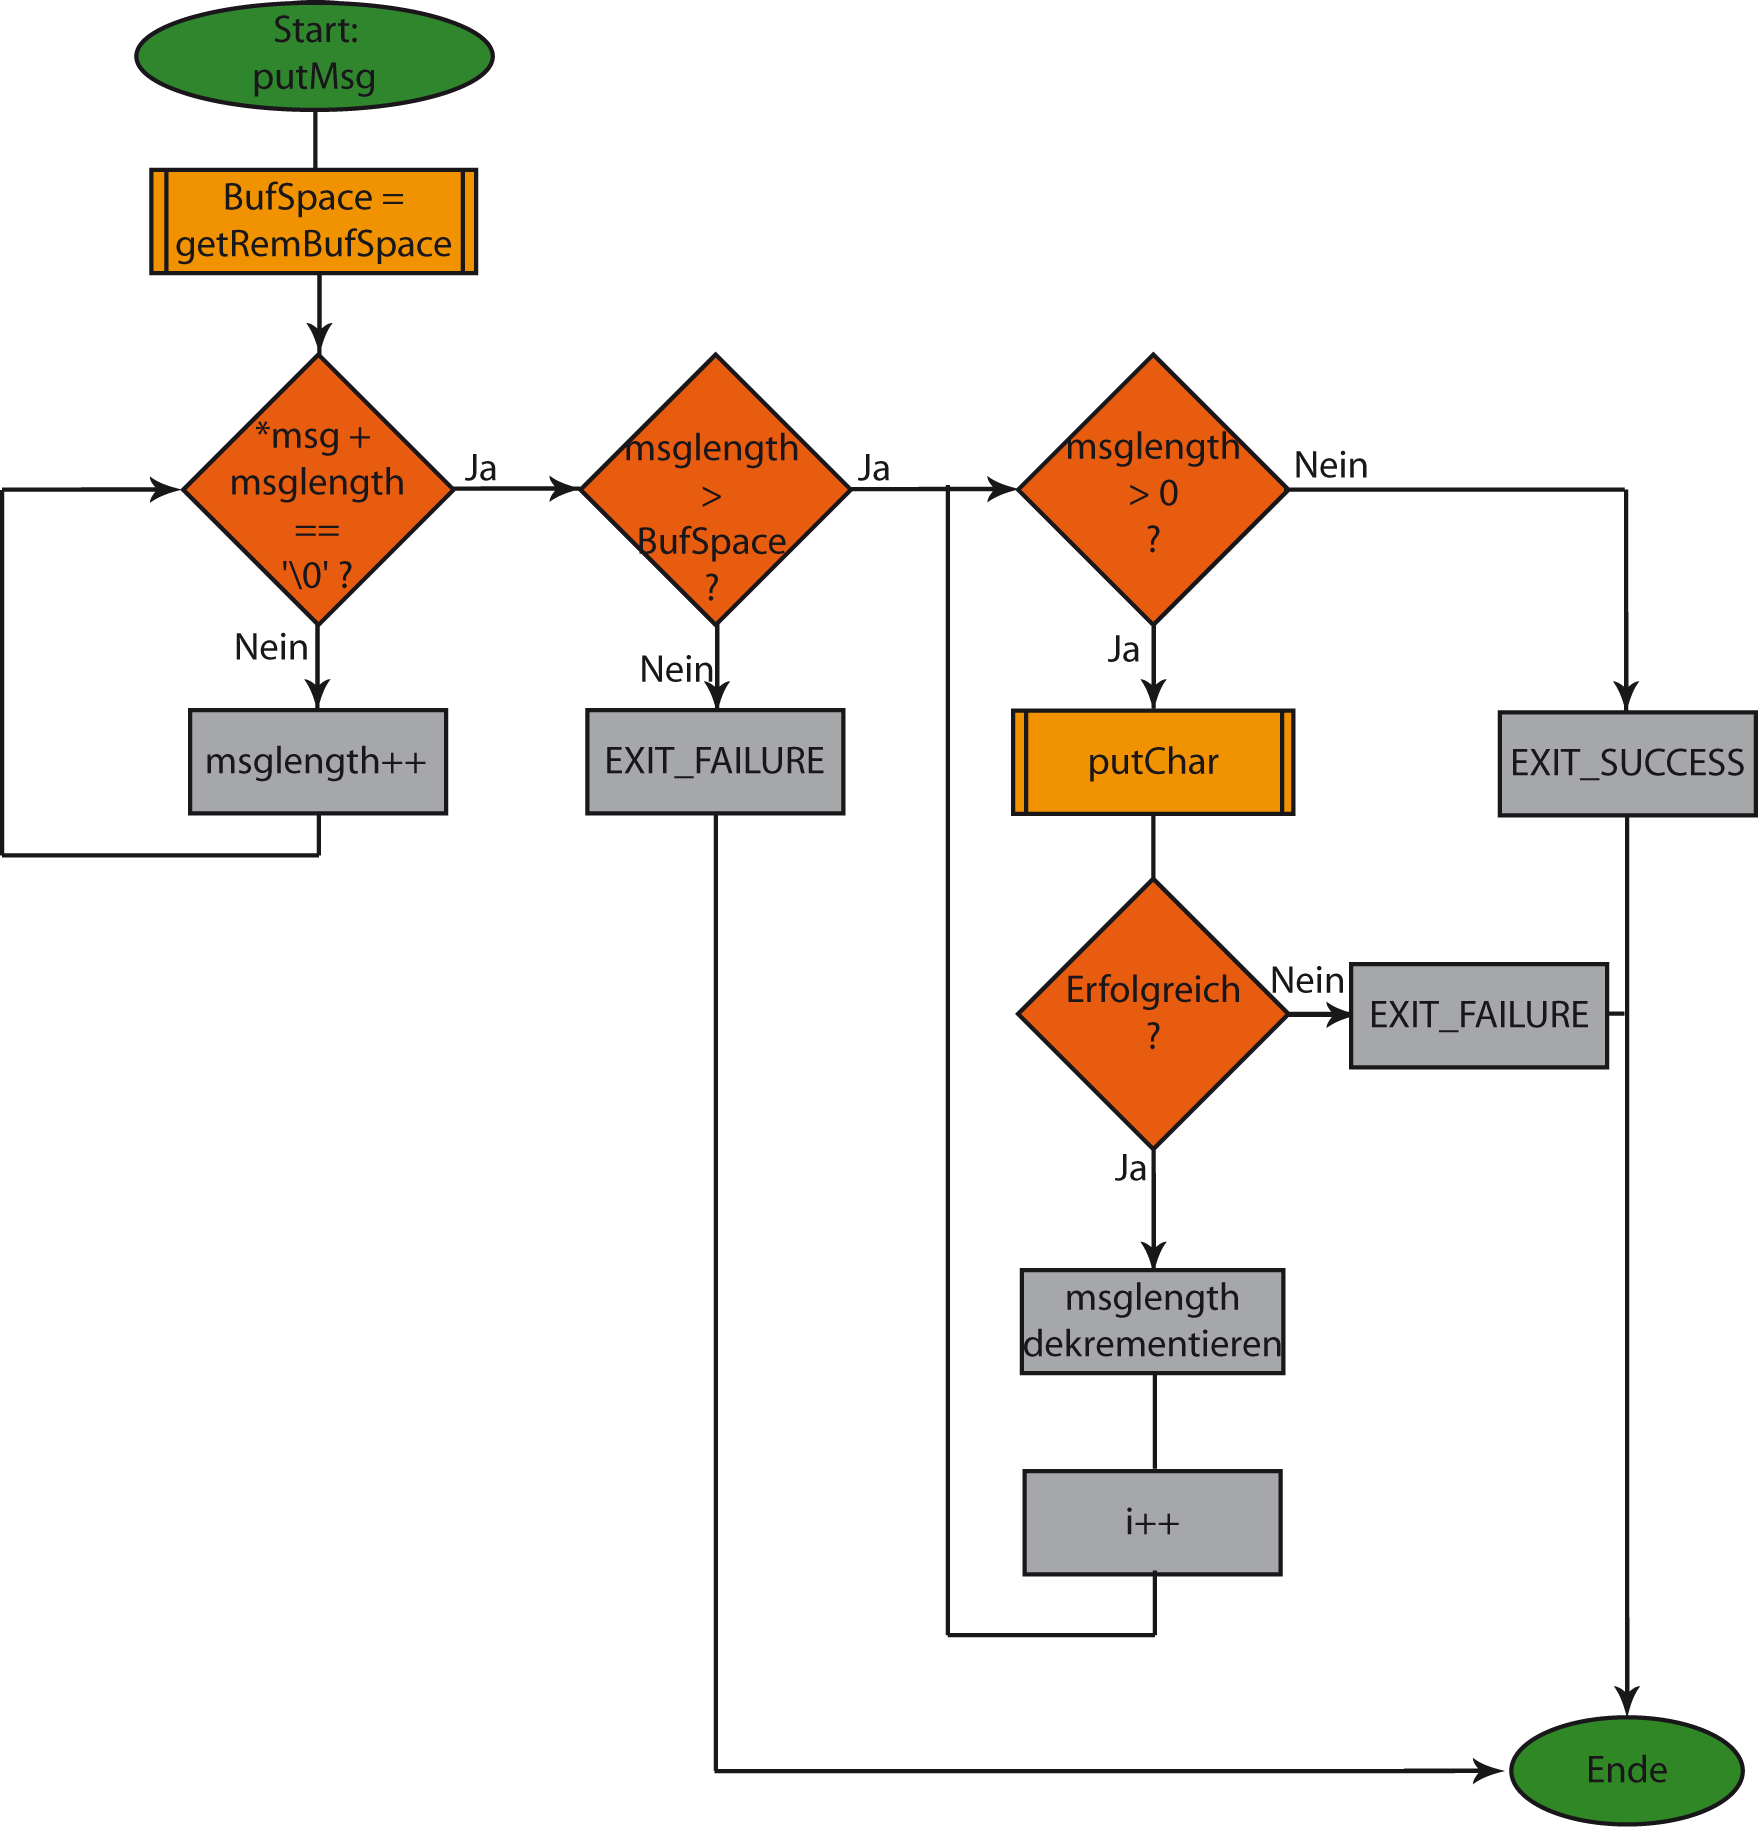
\includegraphics[scale = 0.8]{./putMsg.png}
\hspace{-14pt}
\caption{Ablaufdiagramm der Funktion putMsg}
\end{figure} 

\begin{figure}[h]
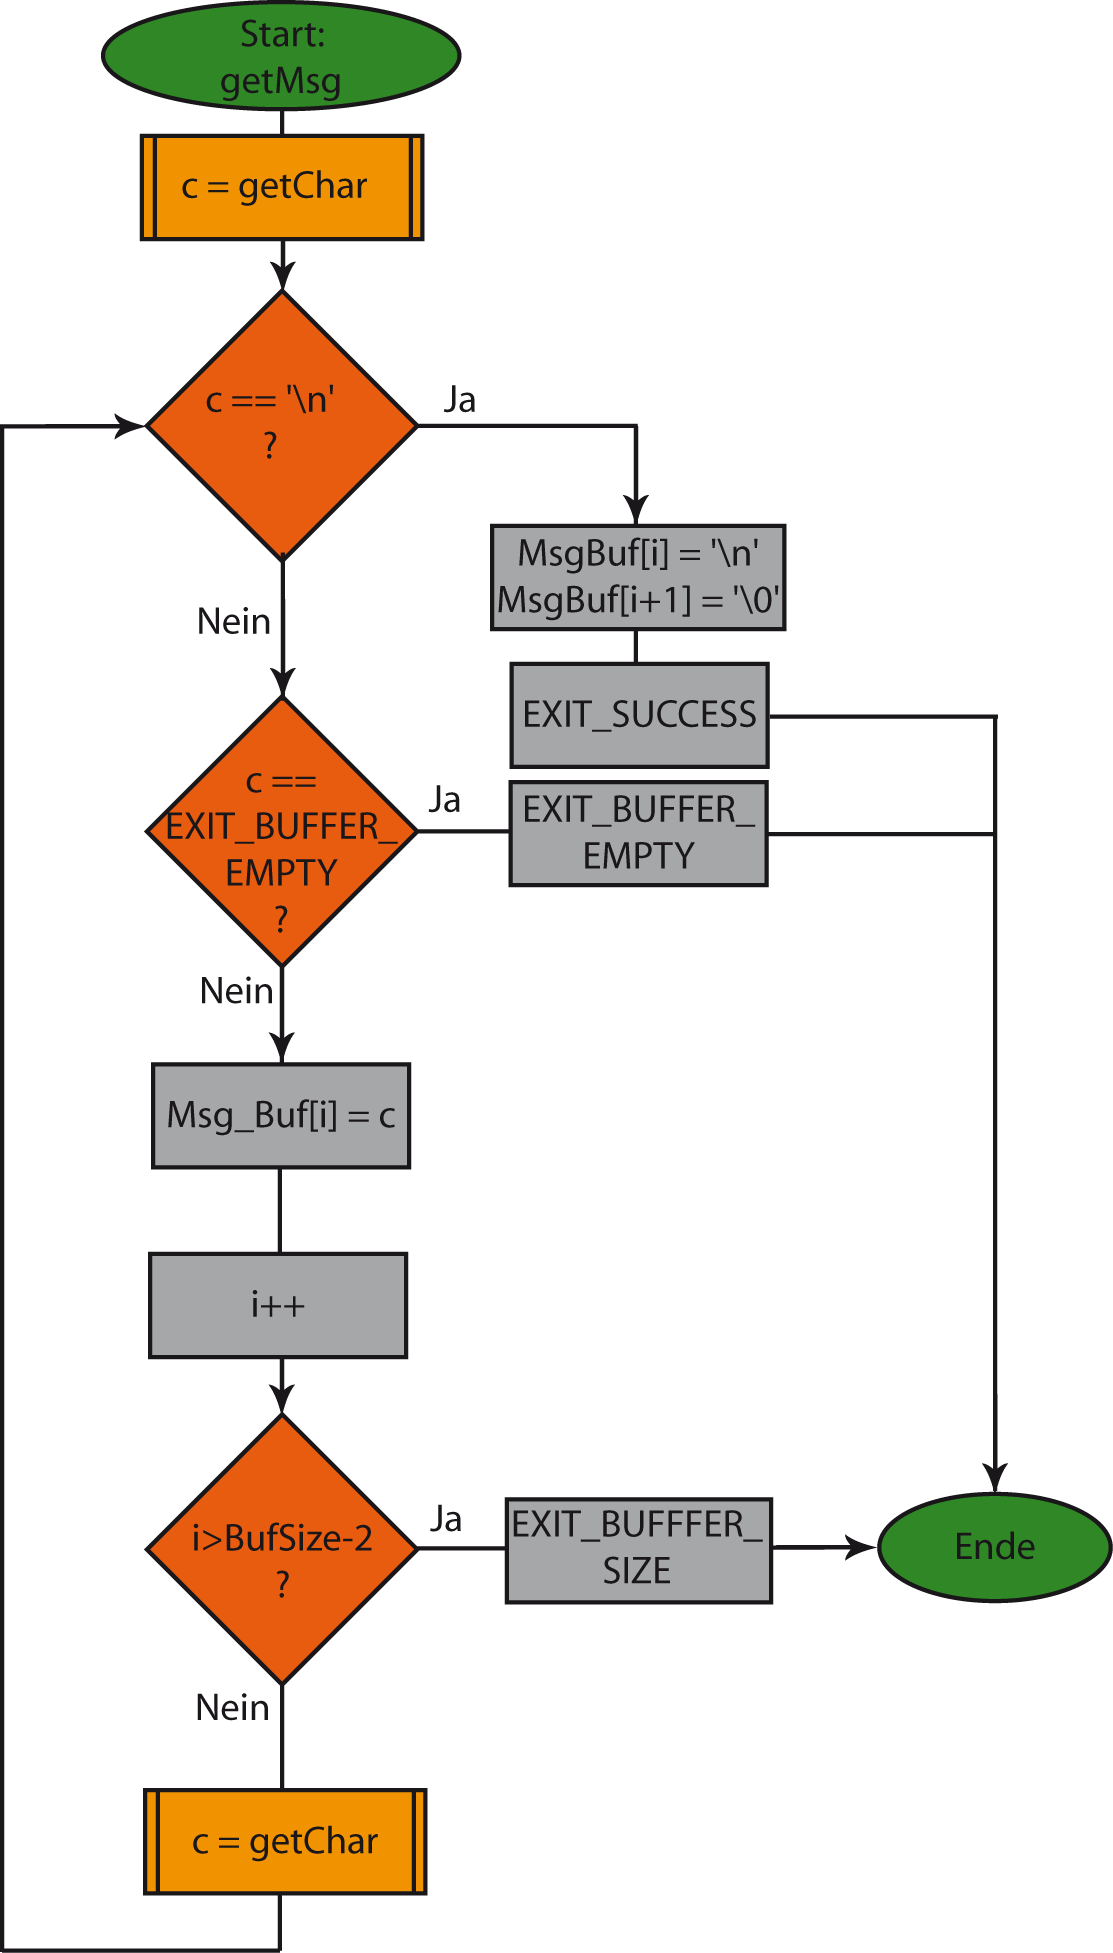
\includegraphics[scale = 0.8]{./getMsg.png}
\hspace{-14pt}
\caption{Ablaufdiagramm der Funktion getMsg}
\end{figure} 








\subsection{inc\_circular.h}
\lstinputlisting{ProjArbBautAutomat-master/inc/inc_circular.h}









\subsection{msg.c}
\lstinputlisting{ProjArbBautAutomat-master/src/msg.c}

\begin{figure}[h]
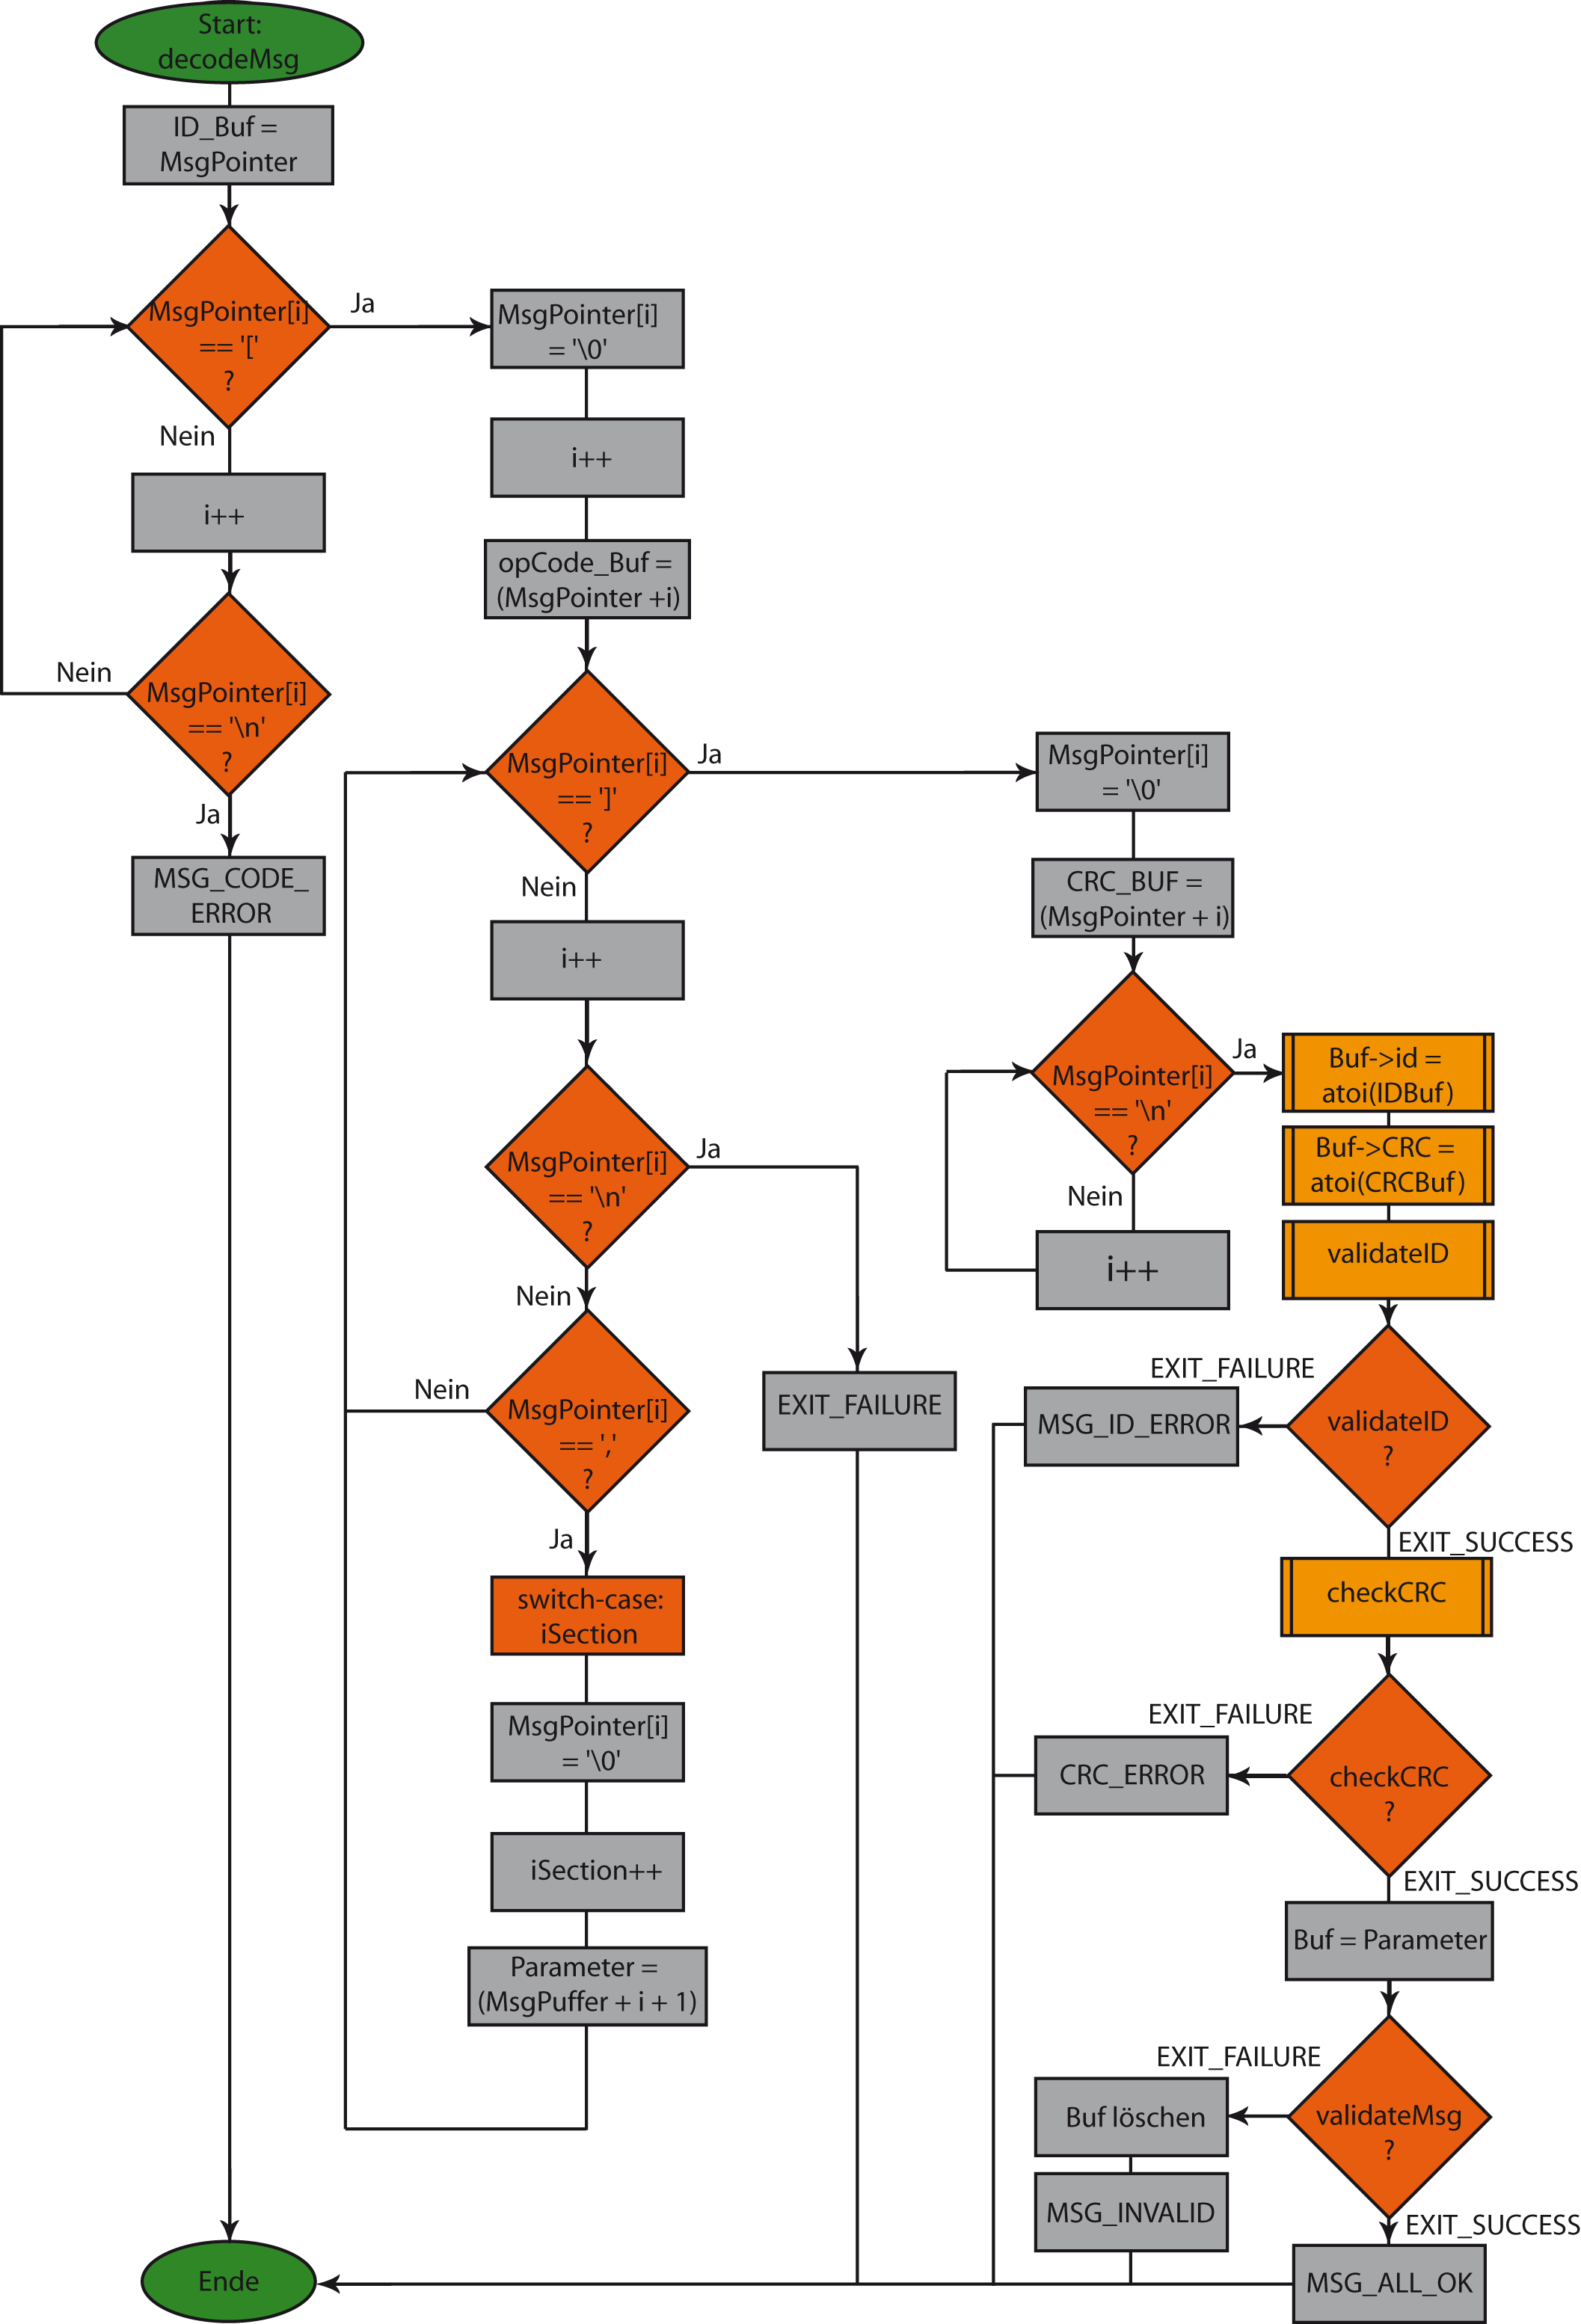
\includegraphics[scale = 0.8]{./decodeMsg.png}
\hspace{-14pt}
\caption{Ablaufdiagramm der Funktion decodeMsg}
\end{figure} 

\begin{figure}[h]
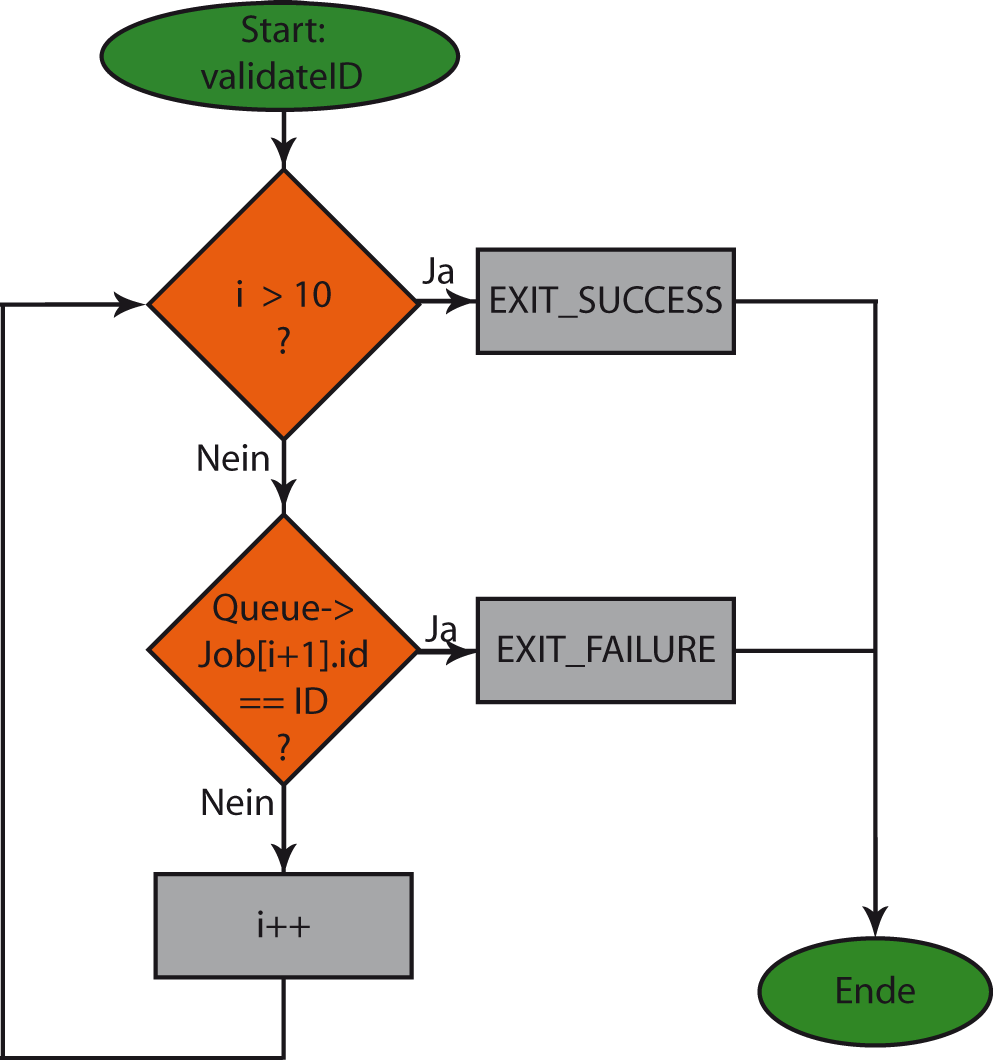
\includegraphics[scale = 0.8]{./validateID.png}
\hspace{-14pt}
\caption{Ablaufdiagramm der Funktion validateID}
\end{figure} 

\begin{figure}[h]
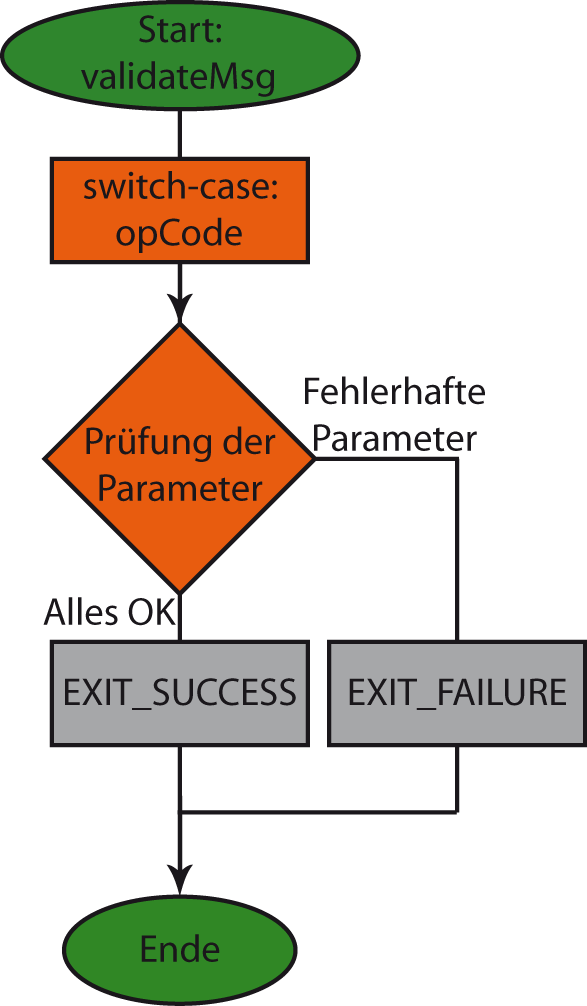
\includegraphics[scale = 0.8]{./validateMsg.png}
\hspace{-14pt}
\caption{Ablaufdiagramm der Funktion validateMsg}
\end{figure} 

\begin{figure}[h]
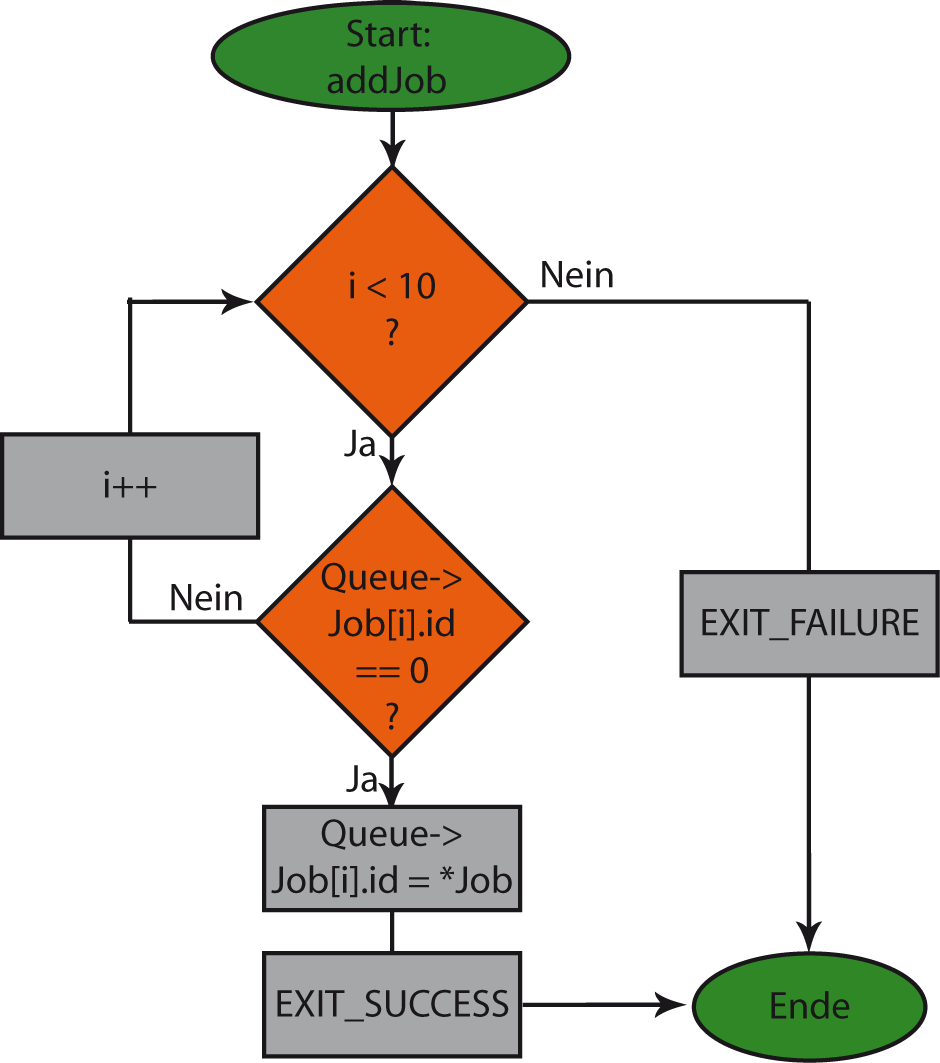
\includegraphics[scale = 0.8]{./addJob.png}
\hspace{-14pt}
\caption{Ablaufdiagramm der Funktion addJob}
\end{figure} 

\begin{figure}[h]
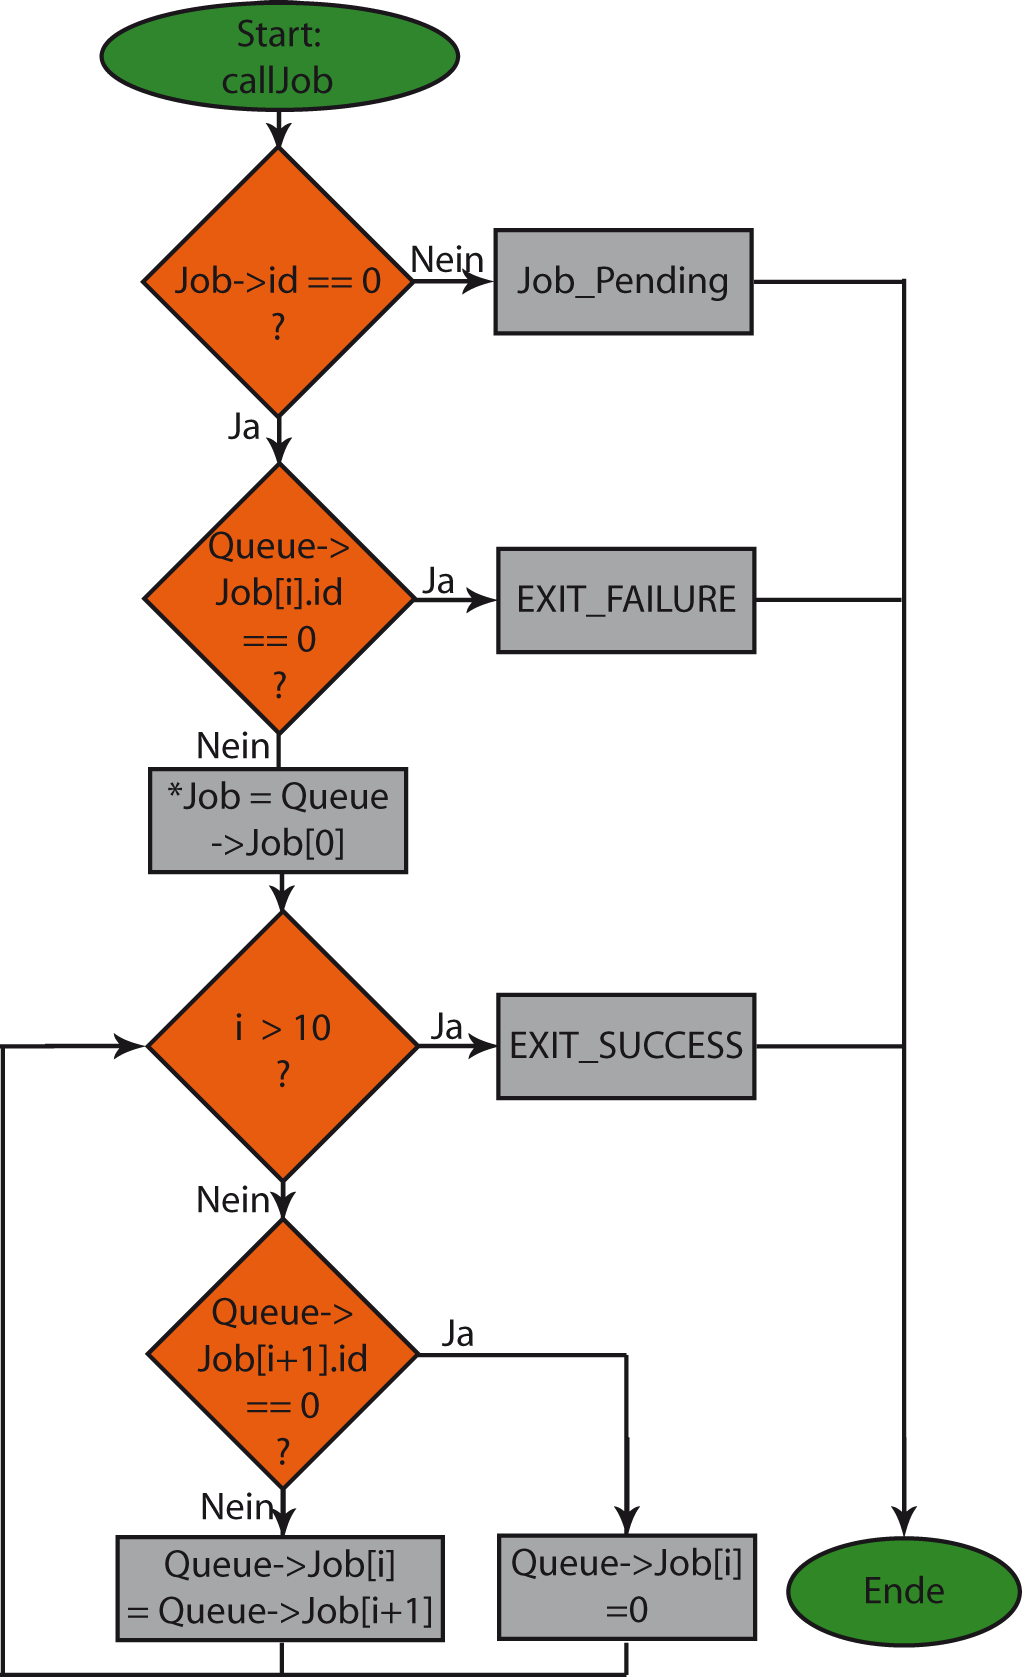
\includegraphics[scale = 0.8]{./callJob.png}
\hspace{-14pt}
\caption{Ablaufdiagramm der Funktion callJob}
\end{figure} 





\subsection{inc\_msg.h}
\lstinputlisting{ProjArbBautAutomat-master/inc/inc_msg.h}





\subsection{motor.c}
\lstinputlisting{ProjArbBautAutomat-master/src/motor.c}

\begin{figure}[h]
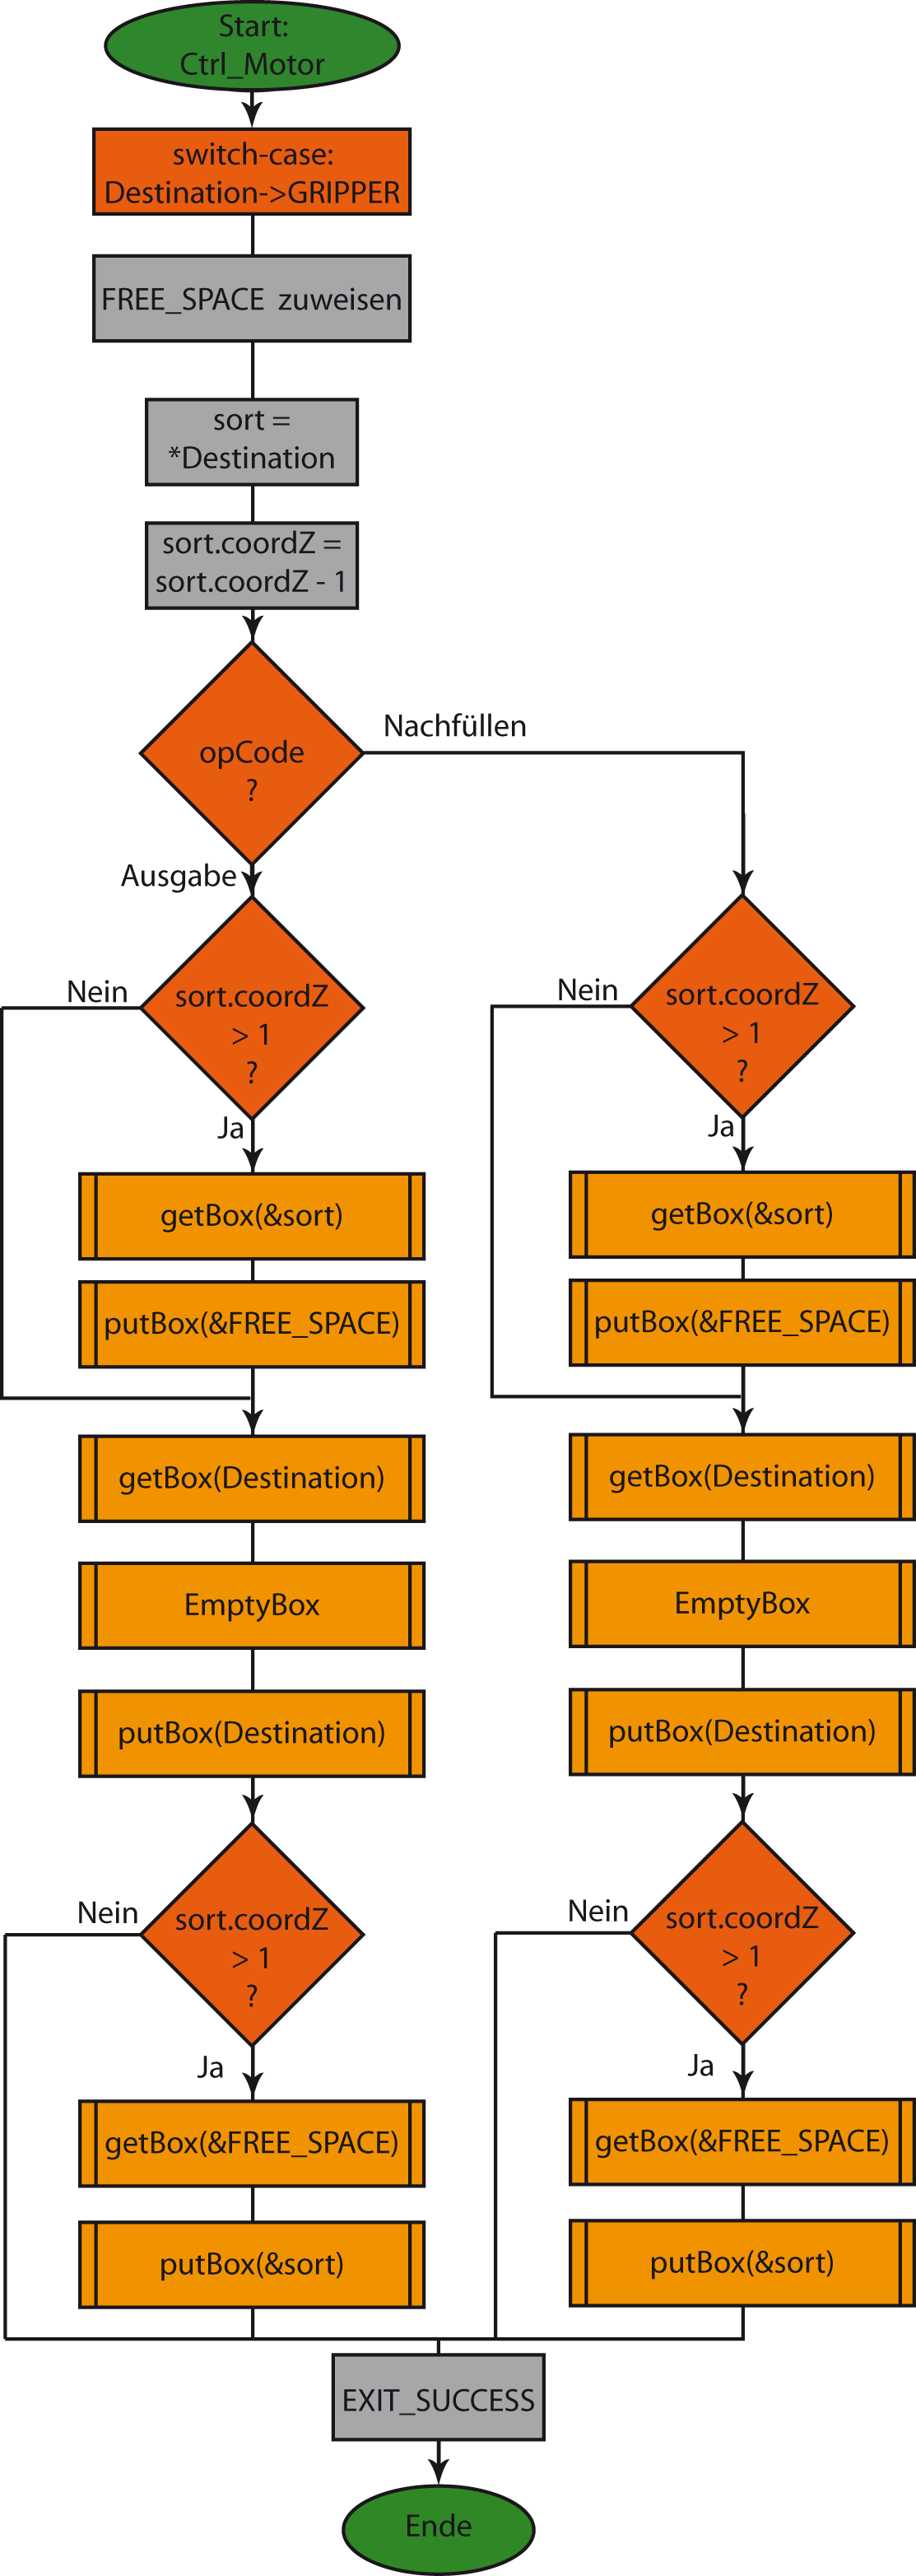
\includegraphics[scale = 0.8]{./Ctrl_Motor.png}
\hspace{-14pt}
\caption{Ablaufdiagramm der Funktion Ctrl\_Motor}
\end{figure} 

\begin{figure}[h]
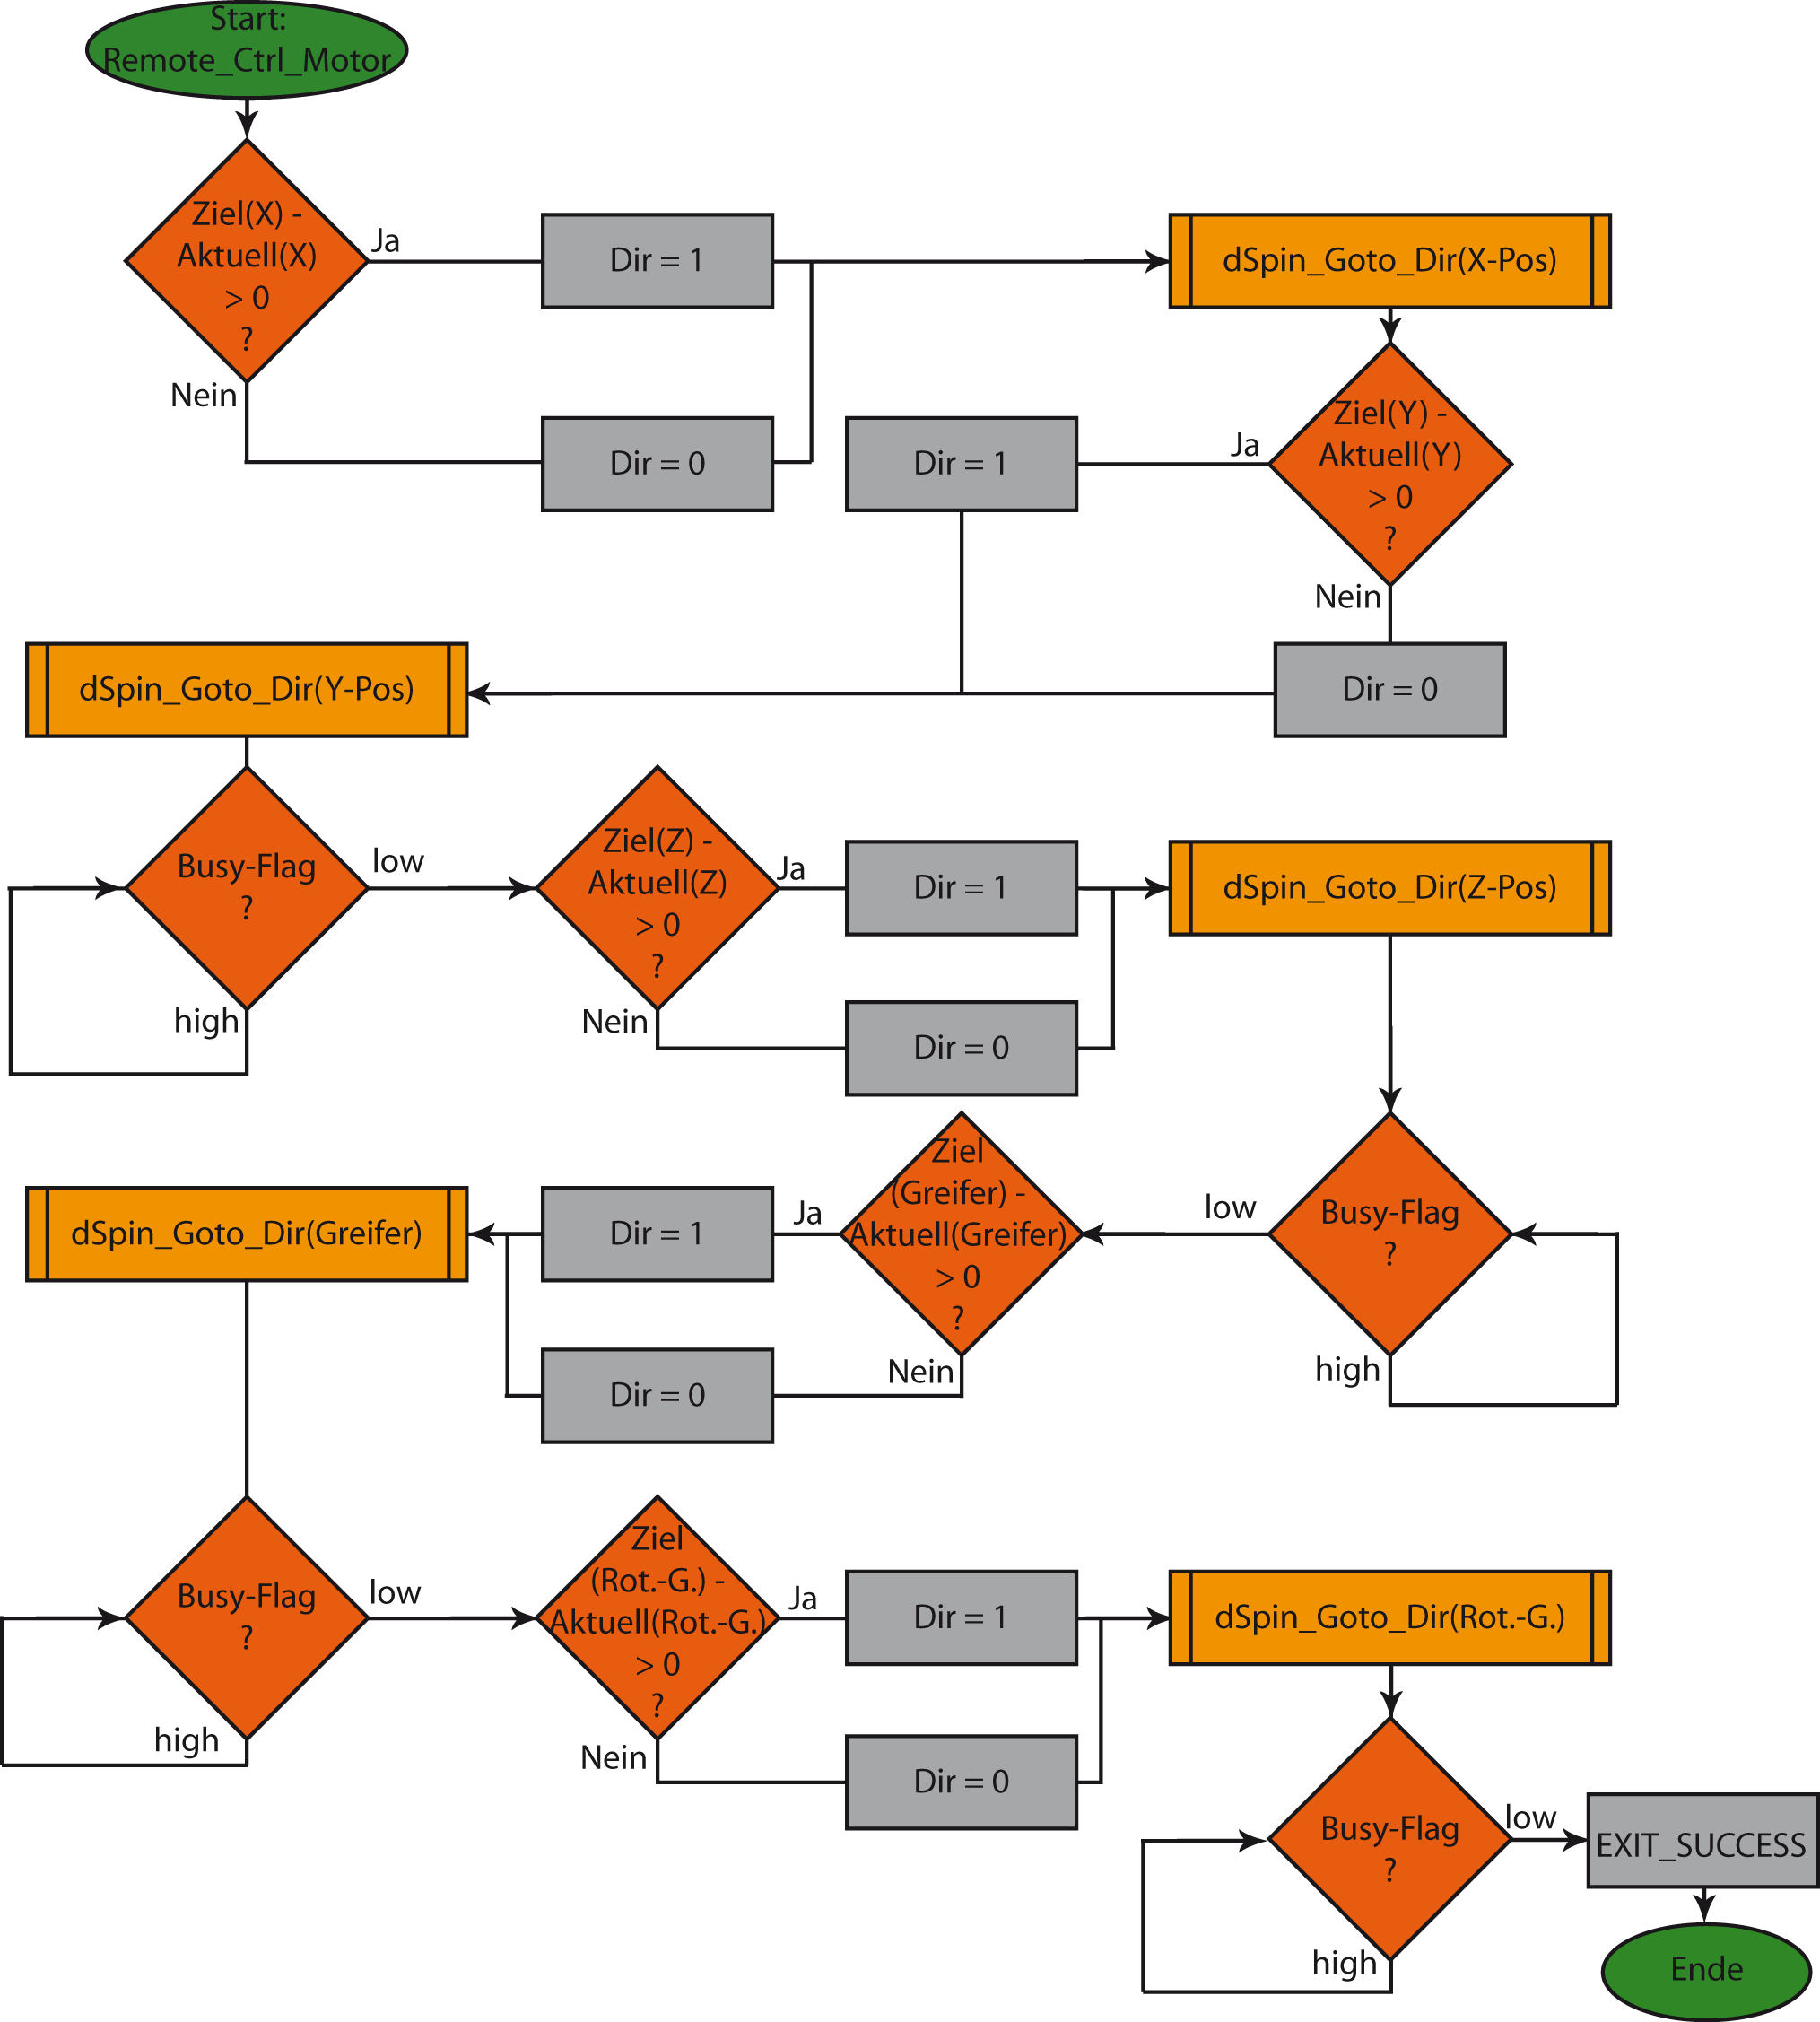
\includegraphics[scale = 0.8]{./Remote_Control_Motor.png}
\hspace{-14pt}
\caption{Ablaufdiagramm der Funktion Remote\_Ctrl\_Motor}
\end{figure} 

\begin{figure}[h]
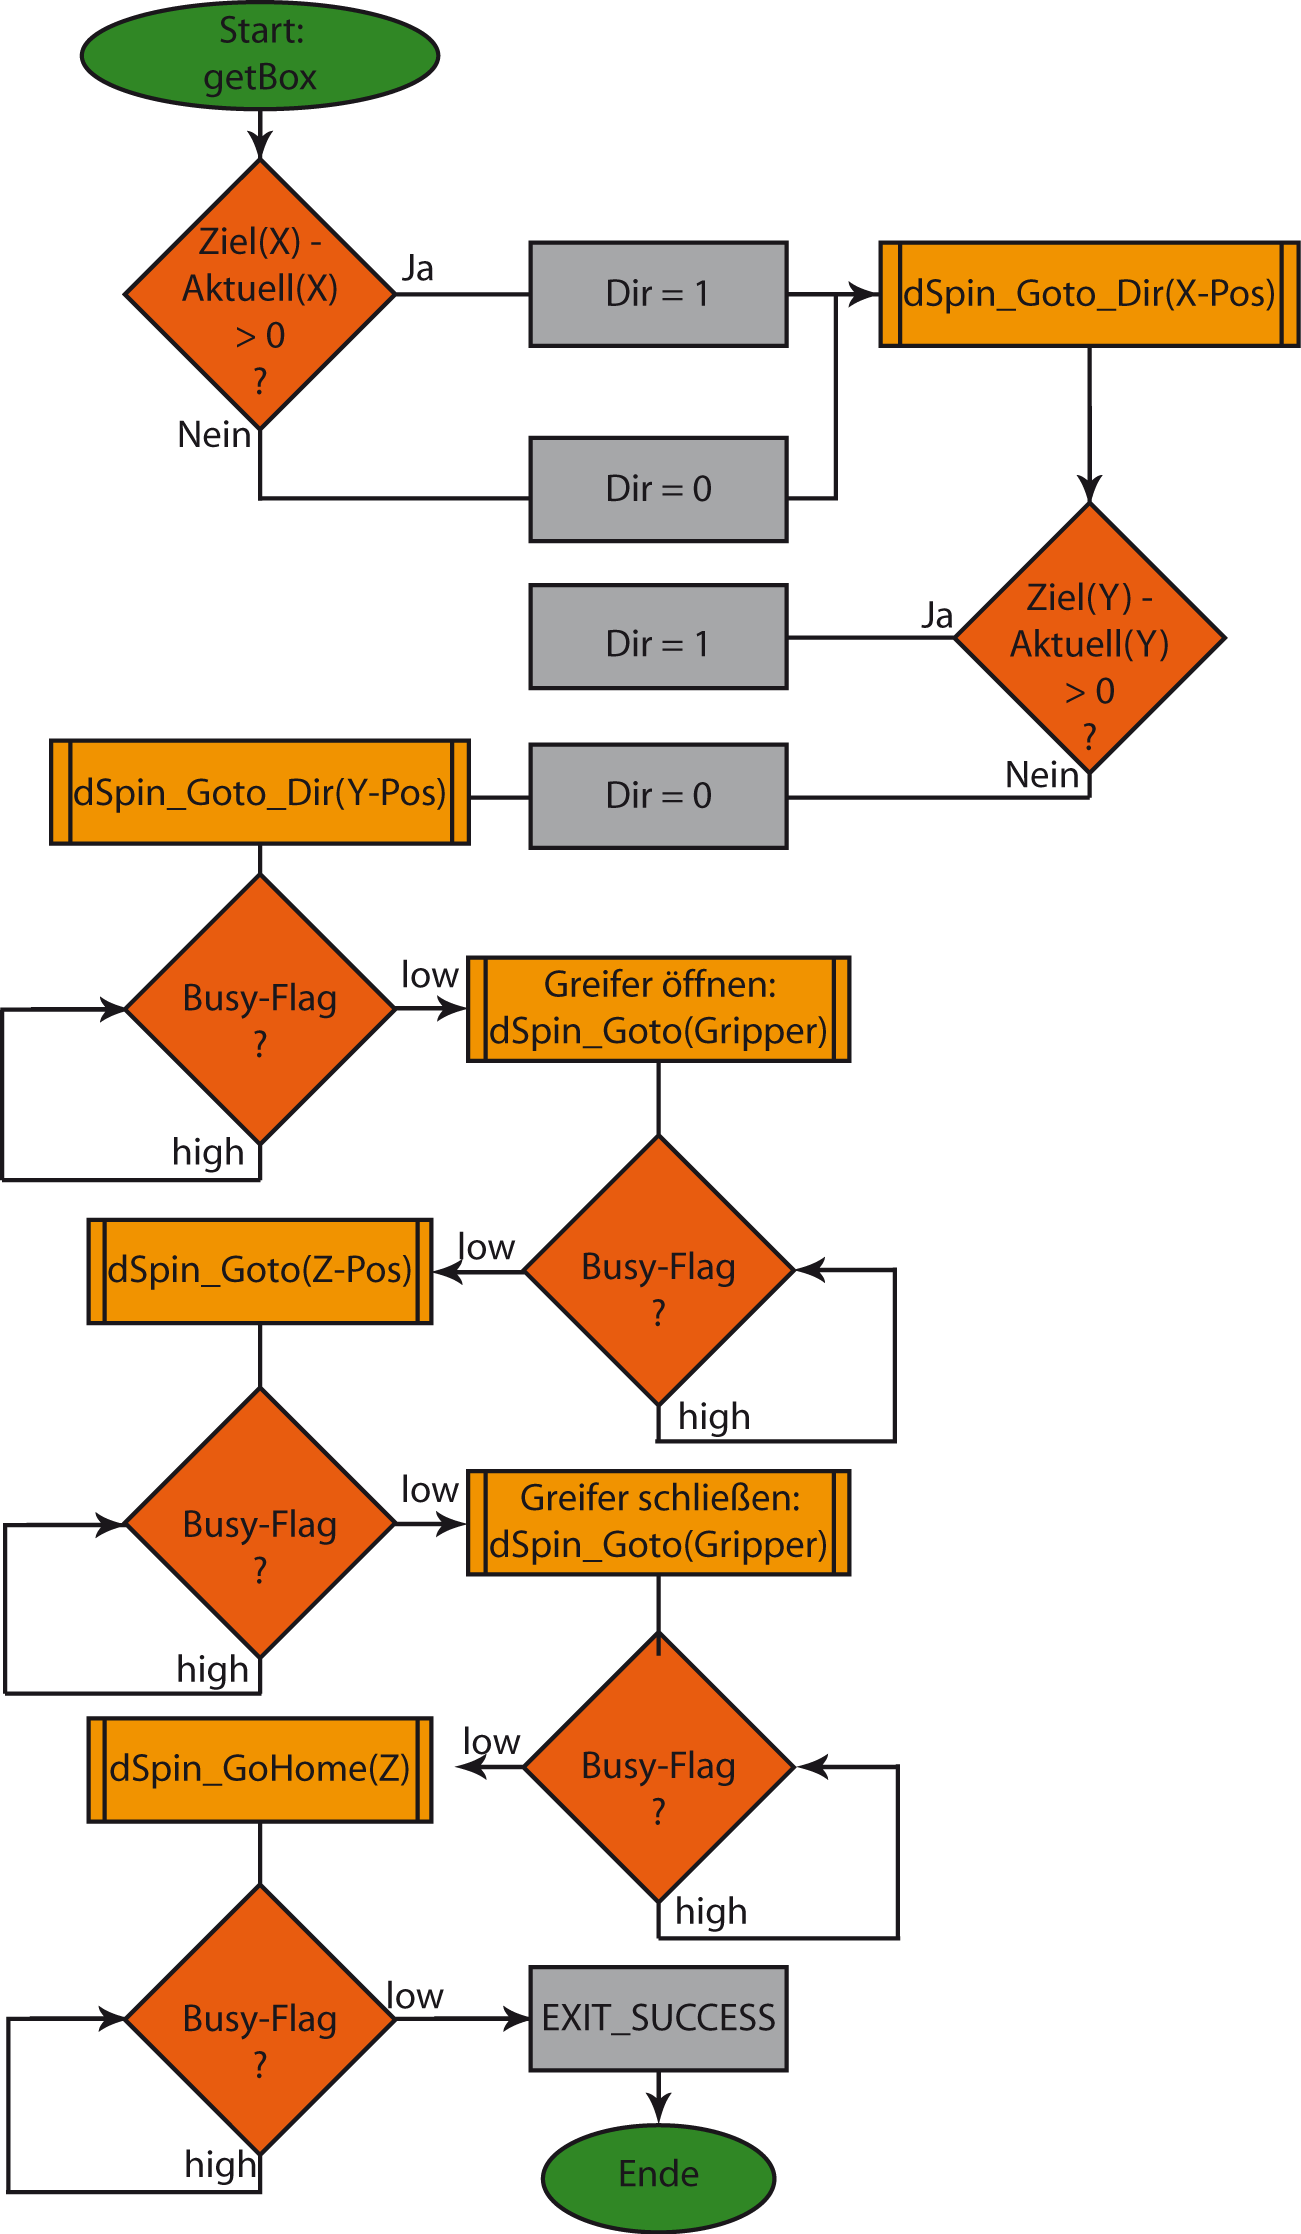
\includegraphics[scale = 0.8]{./getBox.png}
\hspace{-14pt}
\caption{Ablaufdiagramm der Funktion getBox}
\end{figure} 

\begin{figure}[h]
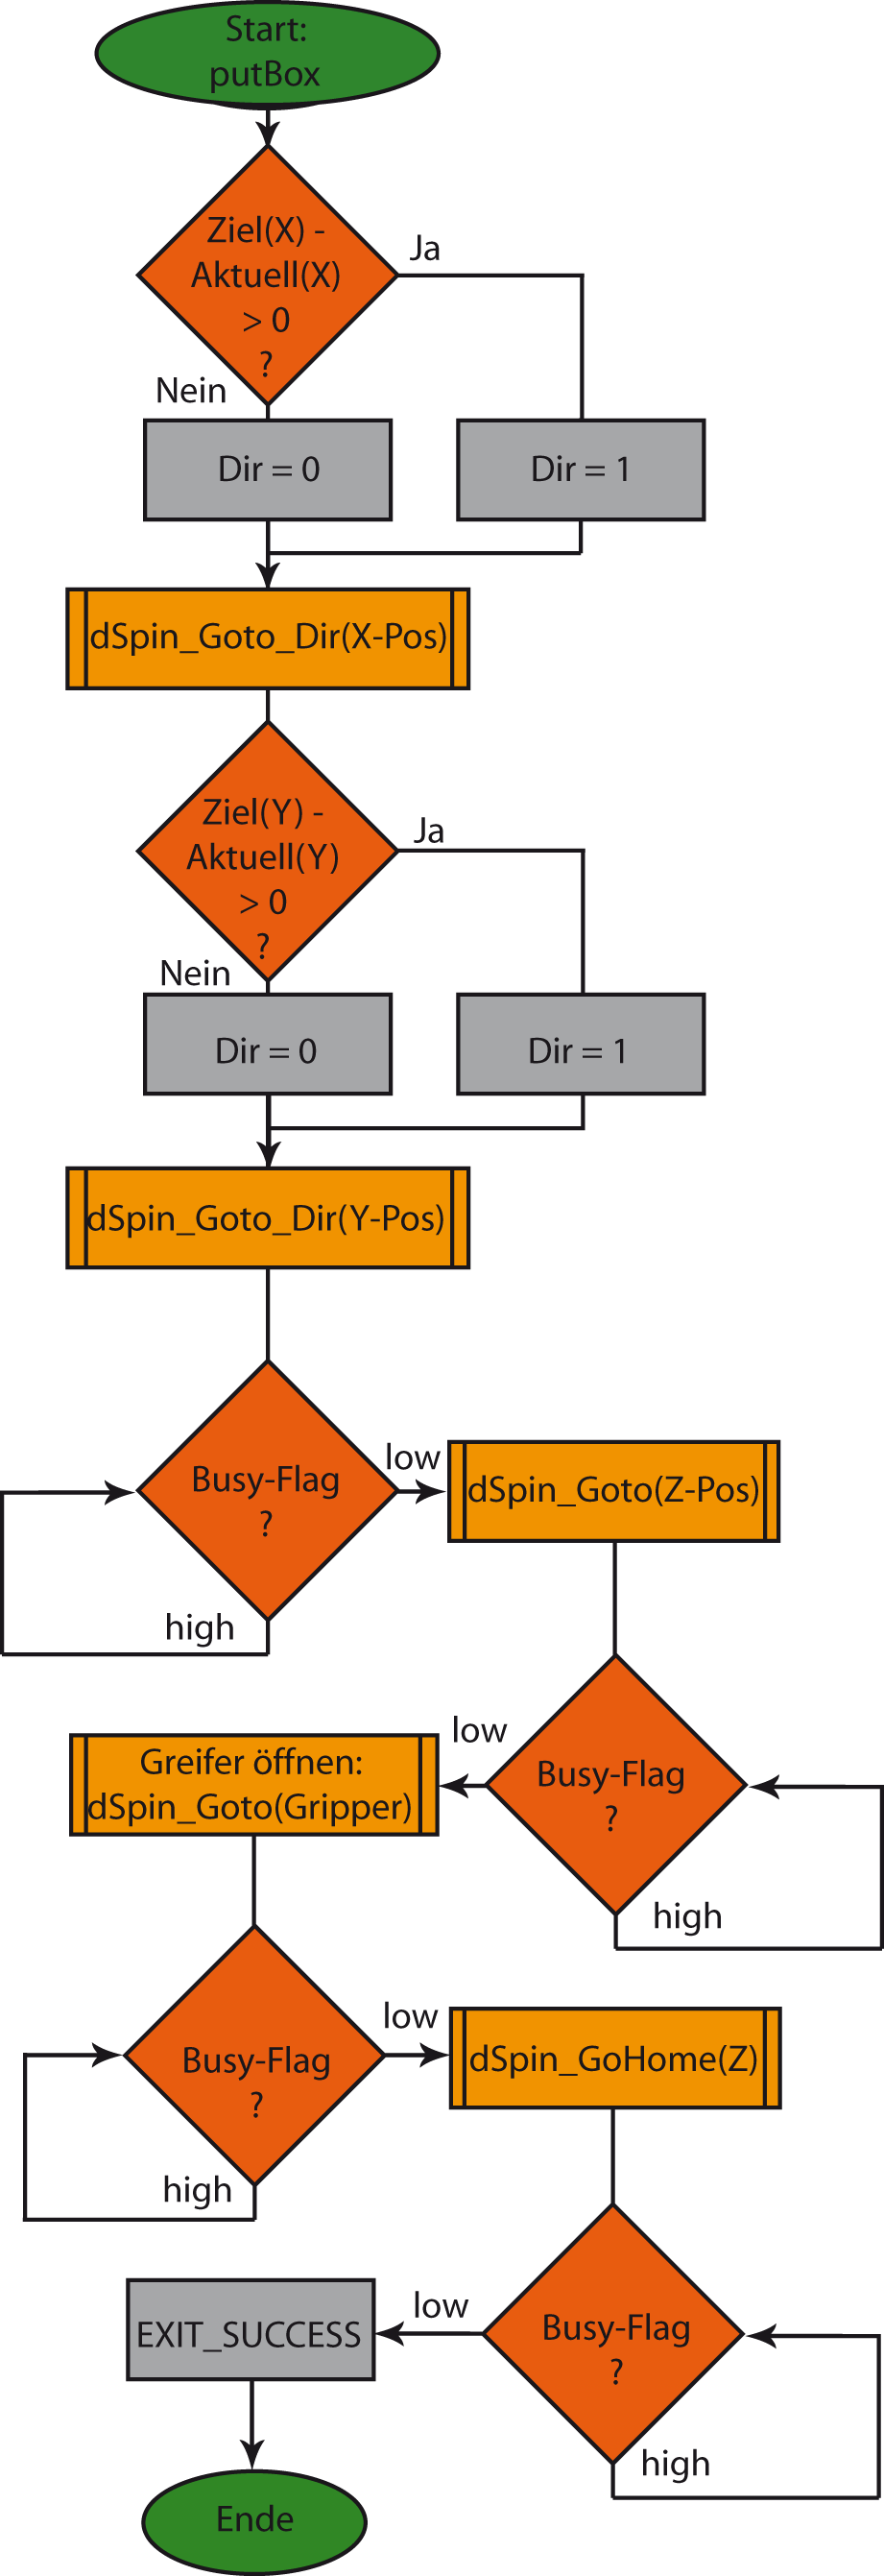
\includegraphics[scale = 0.8]{./putBox.png}
\hspace{-14pt}
\caption{Ablaufdiagramm der Funktion putBox}
\end{figure} 

\begin{figure}[h]
\includegraphics[scale = 0.8]{./EmptyBox.png}
\hspace{-14pt}
\caption{Ablaufdiagramm der Funktion EmptyBox}
\end{figure} 

\begin{figure}[h]
\includegraphics[scale = 0.8]{./RefillBox.png}
\hspace{-14pt}
\caption{Ablaufdiagramm der Funktion RefillBox}
\end{figure} 





\subsection{inc\_motor.h}
\lstinputlisting{ProjArbBautAutomat-master/inc/inc_motor.h}

\subsection{def.c}
\lstinputlisting{ProjArbBautAutomat-master/src/def.c}

\subsection{inc\_def.h}
\lstinputlisting{ProjArbBautAutomat-master/inc/inc_def.h}

\subsection{startup.c}
\lstinputlisting{ProjArbBautAutomat-master/src/startup.c}

\subsection{inc\_startup.h}
\lstinputlisting{ProjArbBautAutomat-master/inc/inc_startup.h}
